\documentclass[12pt, block=fill]{beamer}
\usepackage{graphicx}
\usepackage[sfdefault]{FiraSans}
\usepackage{FiraMono}
\usepackage[T1]{fontenc}
\usepackage{xcolor}
\usepackage{mathtools}
\usepackage{relsize}
\usepackage{tikz}
\usetikzlibrary{arrows,shapes}

\usepackage{hyperref}
\usepackage{tabularx}

\definecolor{burntOrange}{rgb}{.8, .5, .1}
\definecolor{textgray}{rgb}{.8,.8,.8}
\definecolor{berkeleyYellow}{HTML}{FDB515}

\newcommand{\alex}[1]{\textcolor{berkeleyYellow}{#1}}
\newcommand{\paul}[1]{\textcolor{red}{#1}}

\usetheme[
titleformat frame = smallcaps,
subsectionpage = progressbar]
{metropolis}

\metroset{
  block=fill
}

\newcommand{\E}{\text{E}}
\newcommand{\V}{\text{V}}
\newcommand{\cov}{\text{cov}}
\newcommand{\Z}{\mathbb{Z}}
\newcommand{\R}{\mathbb{R}}
\newcommand{\N}{\mathbb{N}}
\newcommand{\indep}{\mathrel{\text{\scalebox{1.07}{$\perp\mkern-10mu\perp$}}}}

\newcommand{\bluecheck}{}%
\DeclareRobustCommand{\greencheck}{%
  \tikz\fill[scale=0.8, color=green]
  (0,.35) -- (.25,0) -- (1,.7) -- (.25,.15) -- cycle;%
}
\usepackage{pifont}
 \newcommand{\xmark}{\textcolor{red}{\ding{55}} }

\usepackage{pgfpages}
\setbeameroption{hide notes} % Only slides
% \setbeameroption{show only notes} % Only notes
  % \setbeameroption{show notes on second screen=right} % Both
\setbeamerfont{note page}{size=\footnotesize}

\title{Week 11}
\subtitle{Questions of Causation}

\author{Paul Laskowski and Alex Hughes}
\institute{UC Berkeley, School of Information}

\begin{document}

\begin{frame}
  \maketitle
\end{frame}

\section{Questions of Causation}

\begin{frame}
  \frametitle{Some Business Questions}
  
  \note[item]{Lets start this week by thinking about some business questions.  here's some...}
\begin{itemize}
\item What will happen to coffee sales if we buy a new roaster?
\item Will profits be higher if we design a new jet or upgrade our existing one?
\item Will more people visit our amusement park if we add a monorail?

 \note[item]{One feature that ties all these questions together is
   that they are causal questions.  Actually, most business questions
   are causal questions.  They are about making a decision or pulling
   a lever.  how can we approach them?  Of course we want to use
   data...} 

\end{itemize}

\end{frame}


\begin{frame}
  \frametitle{Amusement Park Daily Visitors}
  \centering
  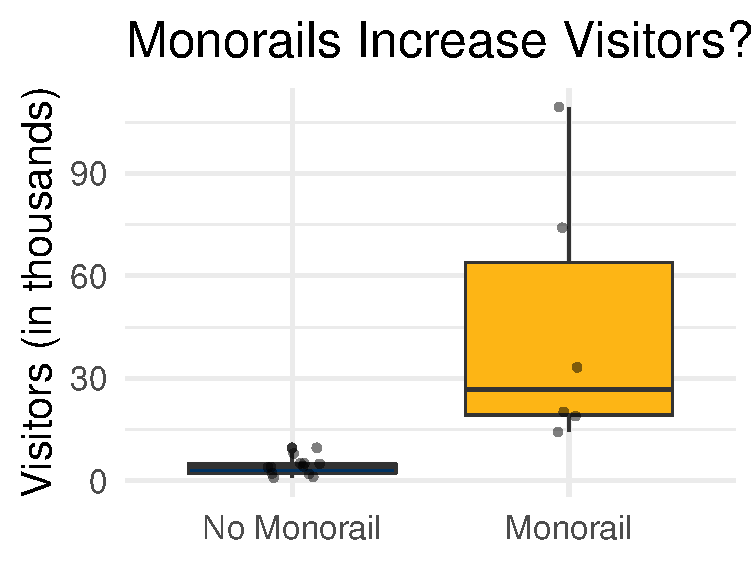
\includegraphics[width = \textwidth]{images/monorail}
  
  
  \note[item]{Here's some data!  You can clearly see that amusement
    parks with monorails get a lot more visitors than amusement parks
    without monorails.  Does that answer your question?}
  \note[item]{Well, not really.  your question is not about the
    distribution of amusement parks, it's about a single amusement
    park.  Or about the process that leads amusement parks to have more or less visitors}
  \note[item]{The question kind of sounds like a prediction problem;
    it kind of sounds like a description problem; but it is
    \textit{different}.} 
  \note[item]{What happens if you change a feature of that one
    datapoint.  Will we really see this huge increase in visitors?
    Maybe and maybe not.}
  \note[item]{This data is certainly relevant, but it's not enough to answer the question.}   
\end{frame}

\begin{frame}
  \frametitle{Amusement Park Daily Visitors (con't)}

  \centering
  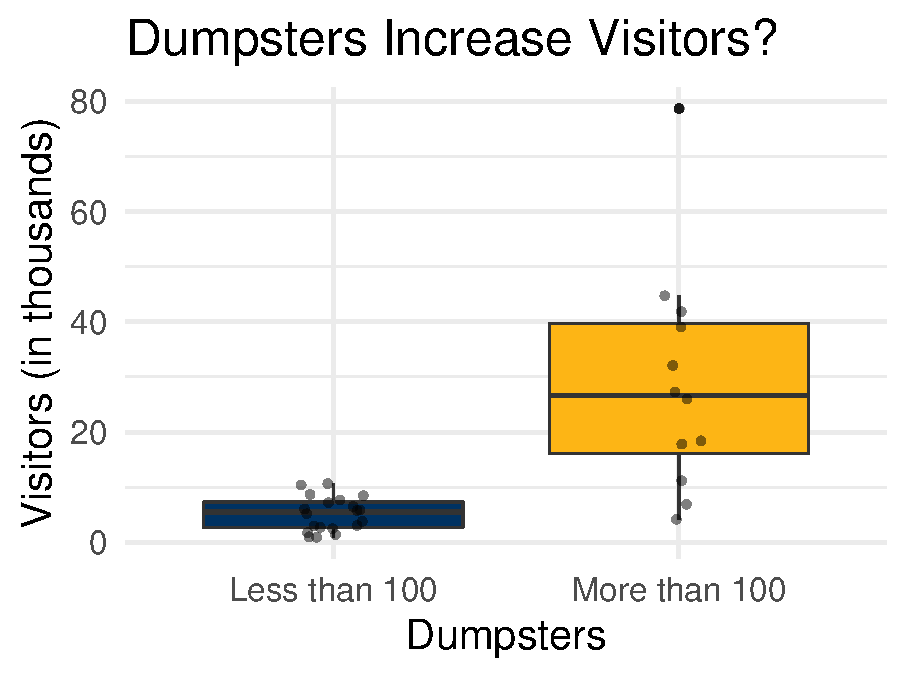
\includegraphics[width=\textwidth]{images/dumpsters}

  \note[item]{If we were to work \textit{only} based on the data,
    then:}
  \note[item]{If we are willing to conclude that monorails increase
    visitors}
  \note[item]{We must also accept that smelly fish guts increase
    visitors.}
  \note[item]{Of corse this isn't the case. There must be something
    else that is \textit{causing} this increase in visitors.} 
\end{frame}

\begin{frame}[standout]

  Correlation $\neq$ Causation
  
  \note[item]{Of course, the problem is that all we can see in our
    graphs and our tables is that a correlation exists.}
  \note[item]{And as I know you've heard many many times...}
  

  \note[item]{So just because monorails are correlated with visitors,
    that doesn't mean that monorails cause visitors; the same with
    dumpsters.}
  \note[item]{There could be many other explanations.}
  \note[item]{I know this might seem really basic. But really it's a
    mistake that many people and businesses make.}
  \note[item]{Example 1: ``What if'' analysis tool at [Company]}
  \note[item]{Example 2: Every Dashboard.}
  \note[item]{Test Prep services.} 


\end{frame}

\begin{frame}
\note[item]{In this unit, we're going to look at explanatory modeling, which
  is a branch of data science that attempts to answer causal
  questions.} 

\center{\textbf{Explanatory modeling:} How can we test or estimate an
  effect in a causal theory?} 
\end{frame}



\section{Unit Plan}

\begin{frame}
  \frametitle{Plan for the Week}
  Three sections
  \begin{enumerate}
  \item What is explanatory modeling?
  \item The one-equation structural model
  \item Common violations of the one-equation model
  \begin{itemize}
\item Confounding, omitted variable bias
\item Outcome on the RHS
\item Simultaneity bias
\end{itemize}

\end{enumerate}

  \note[item]{}
\end{frame}

\begin{frame}
  \frametitle{Plan for the Week (cont.)}
  At the end of this week, you will be able to:
  \begin{itemize}
  \item Recognize major strategies for estimating causal effects
  \item Understand the assumptions behind the one-equation structural model
  \item Reason about common violations of the one-equation structural model
  \end{itemize}
\end{frame}

\section{What Is Explanatory Modeling?}

\begin{frame}
  \frametitle{Toward Explanation}
  \note[item]{Let's discuss what explanatory modeling is.}
  \note[item]{We know that we want to measure causal effects.}
  \note[item]{There's a question that a lot of students have at this
    point, and it goes like this} 
  \vspace{1.5cm}
  
  What extra assumptions are needed for OLS regression coefficients to be causal?*
  
  \vspace{2cm}
  
  \flushright * Misleading question
  
  \note[item]{Well, I'm here to tell you that this isn't the best question.}
  \note[item]{It's not technically wrong, but it makes it sound like you
    can transform a descriptive model into a causal model.}
  \note[item]{It's a little like asking: What extra assumptions do I need for this
    parachute to work?  The parachute must be designed from the very beginning to slow your descent.} 
  \note[item]{A lot of econometrics textbooks sound like this.  You
    start from an OLS regression and guess what!  You're modeling
    causality! Now you might have to fix a few issues before you can
    publish.} 
  \note[item]{This type of narrative blurs the
    distinction between descriptive and explanatory modeling.   But as a data
    scientist, you need a very clear understanding of both modes --
    because there is a tendency for descriptive models to be read as causal.} 
\end{frame}


\begin{frame}
  \frametitle{The Explanatory Modeling Workflow}

  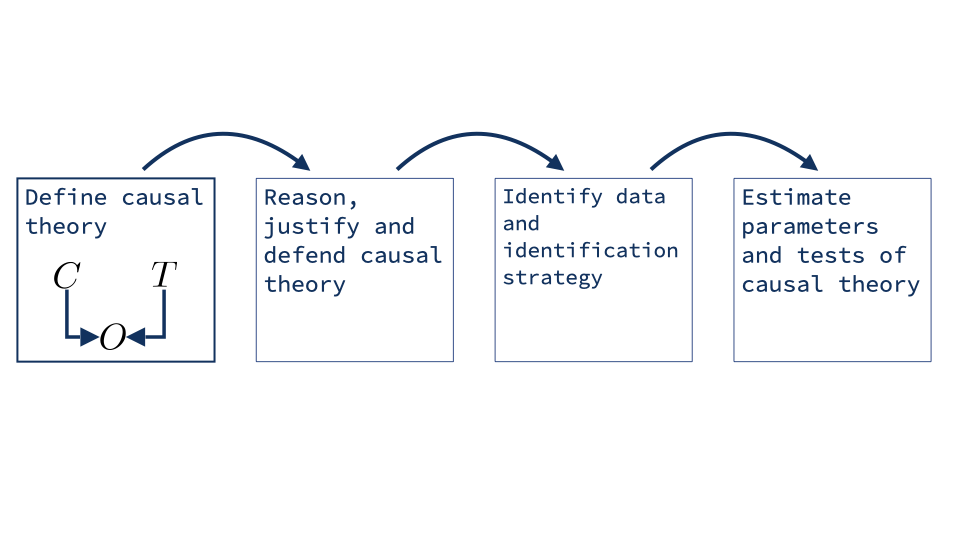
\includegraphics[width = \textwidth]{images/explanatory_workflow/explanatory_workflow_001.png}
  
  \note[item]{So what's a better narrative to have in mind? In this diagram, we've tried to distill four steps that go into an explanatory exercise.}
    \note[item]{This is a simplified view.} 
    \note[item]{There is a lot of variety out there - a lab experiment
      is very different than estimating rates of disease transmission
      - but I still think this picture can help you make sense of
      things} 
  \note[item]{First, we have to define a causal theory.  That's always
    the starting point, our analysis takes place inside a theory.} 
  \note[item]{Some theories may be widely accepted, but often we have
    to justify our theory, or parts of it.} 
  \note[item]{Next, we identify a technique for estimation}
  \note[item]{OLS regression is just one possible technique.  we may
    need a different technique or maybe no technique can work.  it
    depends on the causal theory} 
  \note[item]{Finally, we can estimate parameters, or we can test the theory}
  \note[item]{Next, let's take a closer look at each of these steps} 

\end{frame}

\begin{frame}
  \frametitle{The Explanatory Modeling Workflow}
  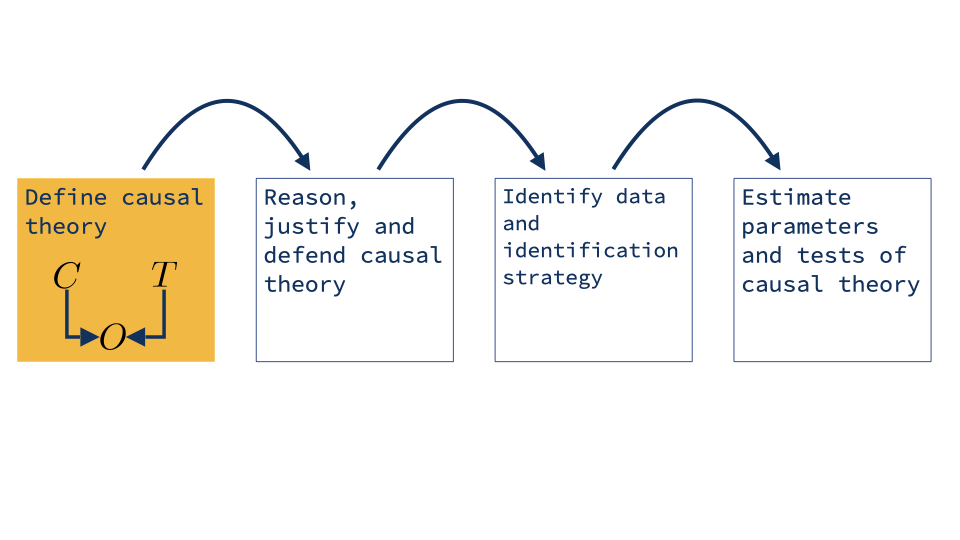
\includegraphics[width = \textwidth]{images/explanatory_workflow/explanatory_workflow_002.png}
\end{frame}


\begin{frame}
  \frametitle{What Is Causal Theory?}

  \note[item]{First to do any explanatory modeling you have to start
    with causal theory.  The word theory might sound scary, but here's what we mean} 

  \begin{block}{Causal theory}
    A \textit{causal theory} is a statement of beliefs about what
    concepts \textit{do} and what concepts \textit{do not} cause other
    concepts.
    % \textbf{Causal theory} - a set of starting assumptions regarding
    % causal relationships.
  \end{block}
      \begin{itemize}

    \item Objective: narrow the range of causal explanations for associations we find in data.
    \end{itemize}

\note[item]{This can come in many forms.  sometimes it's really a
  Theory with a capital 'T'.  other times, it's really just what we
  call background knowledge} 
  \note[item]{You're an engineer, so you know that more horsepower causes a car go faster.  You don't need a fancy theory, you don't even have to stop and think about it, you can just start measuring.}

%\note[item]{By the way, this is something that's really hard for machines to do. The
 % problem space is too unbounded, and the data of the wrong form for
  %them to reason.}

\end{frame}

\begin{frame}
  \frametitle{What is Causal Theory? (cont.)}
   
  \note[item]{Fundamentally, we need some statement about causality to
    begin with, because we can't get from only statements about the
    distribution to statements about causality.}
  
  \begin{itemize}
  \item Joint distributions and cumulative density functions cannot
    identify causal information
  \item If we begin with causal statements, we can use logic to reach causal conclusions
  \end{itemize}
  
  \note[item]{Suppose that you are a part of a data science team that
    is working together with a product team to change the purchase
    flow.}
  \note[item]{You can observe information about your customers, where
    they browse, what they're interested in; and you can
    \textit{posit} some theory -- e.g. when there is \textit{too much
      friction} in the checkout flow, it drives people away.}
  \note[item]{You might have arrived at this idea inductively; you
    might have heard it from the product team; but now you've got to
    ask, ``How can I evaluate whether this theory is useful for
    predicting behavior.'' This is where the experiments come in.}
  \note[item]{You might have noticed that there are seemling byzantine
    tests that are conducted in science -- do we \textit{really} care
    about nutrinos? Yes! They're predicted by theory!} 
  
  \begin{center}
    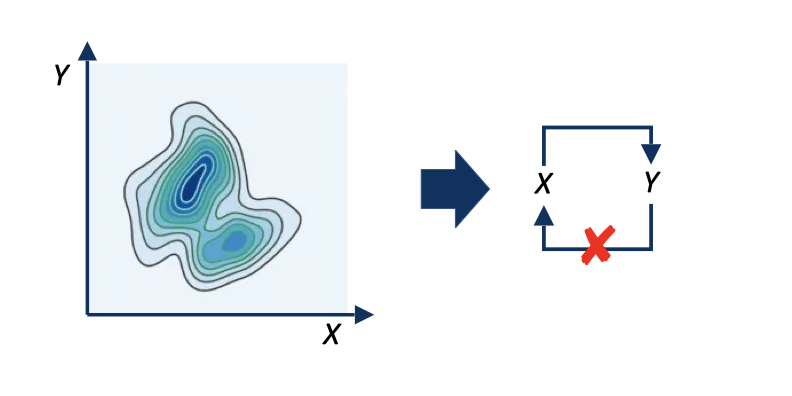
\includegraphics[width = \textwidth]{images/assoc_to_causal.png}
  \end{center} 
  
\end{frame}

\begin{frame}
  \frametitle{How to Reason About a Causal Theory}
  \centering
  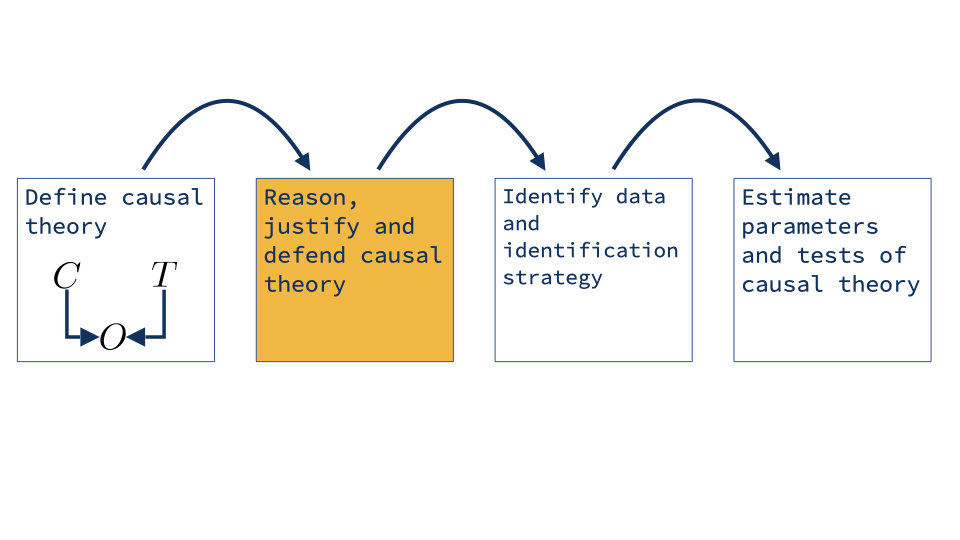
\includegraphics[width = \textwidth]{images/explanatory_workflow/explanatory_workflow_003.png}
\end{frame} 

%\begin{frame}
%  \frametitle{How to Specify a Causal Theory}
% 
% \note[item]{At one extreme is a SEM.  This is where we encode the entire causal system with a set of equations.}
% \note[item]{Here's one classic example: supply and demand.}
% \note[item]{Econ 101 says that as the price of a good goes up, suppliers react by making more of it.  that's the supply curve.  But consumers buy less, so the demand curve slopes down.  The intersection is the equilibrium}
% \note[item]{So we write two equations down  and we assume they both hold at the same time.}
%  
%\textbf{1. Structural Equation Model (SEM)}
%\center 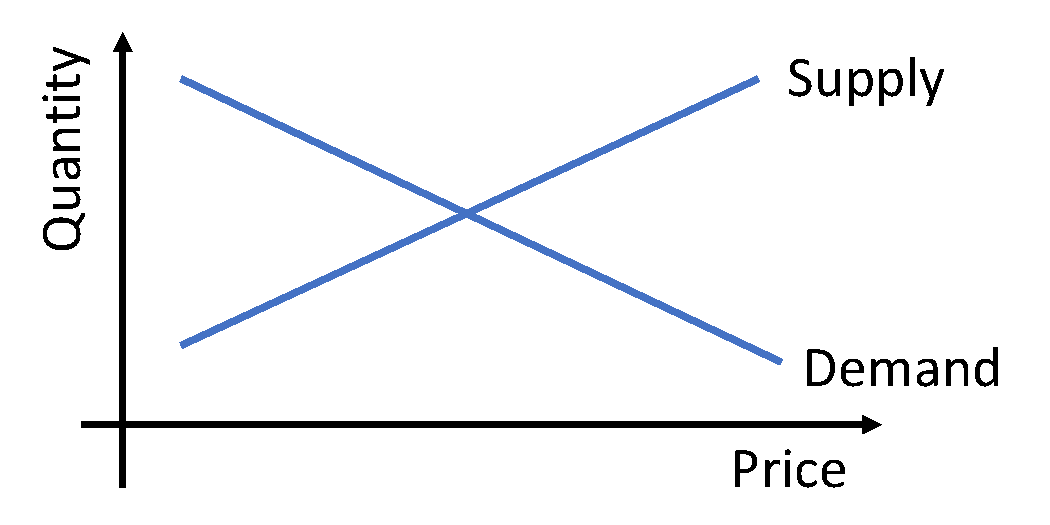
\includegraphics[width = .7\textwidth]{images/supply_demand}
%\begin{align*}
%Demand:  Quantity &= \beta_0 + \beta_1 Price + \epsilon_1\\
%Supply:  Quantity &= \gamma_0 + \gamma_1 Price + \gamma_2 Input\_Costs + \epsilon_2
%\end{align*}
%
%\note[item]{We call these structural equations, because they represent the mechanism that gives rise to the joint distribution.}
%\note[item]{This is a cool idea, and popular in a few place (Penn state is one).  But it's actually not used for very much these days.  The biggest reason is that you have to specify every causal pathway in the system.  How do you convince anyone that your model is right? }
%\note[item]{Also, not every set of equations can be estimated.  In this case, we're lucky, because we have the variable input costs, which only affects supply.  That lets us estimate the slope of the demand curve.  But we may have a hard time finding variables like that.}
%  
%\end{frame}

\begin{frame}
  \frametitle{How to Reason About A Causal Theory (cont.)}

  Creating and eliminating possible causal paths

  \begin{itemize}
  \item \textit{Time structure} 
  \begin{itemize}
\item If $X$ happens after $Y$, then $X$
    cannot have caused $Y$. 
\end{itemize}

  \item \textit{Domain Knowledge}
    \begin{itemize}
    \item Germ theory of infections disease
    \item Often formed through past experiments
    \end{itemize}
  \item \textit{Effectively "random" events}
    \begin{itemize}
    \item Coin flips
    \item Tropical storms
    \item pseudorandom generators
    \end{itemize}
  \end{itemize}
  
  \note[item]{Just like we never are \textit{issued} the joint pdf, we
    are not issued the causal model when we become a data scientist.  How do we get a causal theory?}
  \note[item]{When we start, our default belief will be that \textit{everything}
    causes \textit{everything}.  any causal path could theoretically be there.} 
  \note[item]{Remember that we need to narrow down the range of possible causal explanations.}
  \note[item]{That means we have to eliminate some causal paths. how do we do that?} 
  \note[item]{You might use a coin flip in an experiment to decide who gets a treatment and who gets a placebo.  How do you know that a patient being sick doesn't somehow cause the coin to land heads? If you change the velocity of the coin by even a microscopic amount, it might land a totally different way.  So we believe that the coin is effectively random, nothing else can really cause it to land heads.}
\end{frame}

% ASDF RETURN HERE 

\begin{frame}
  \frametitle{How to Identify an Identification Strategy, Part I}
  \centering
  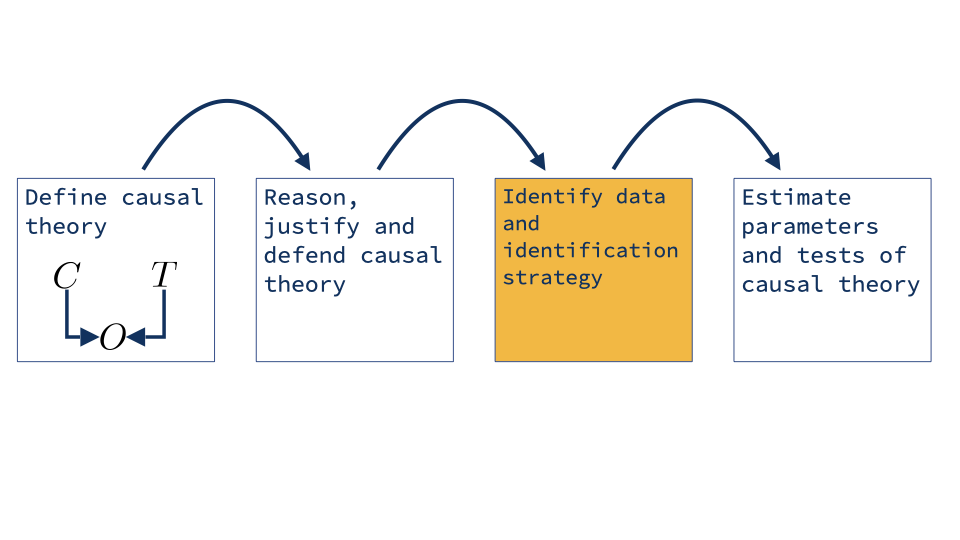
\includegraphics[width = \textwidth]{images/explanatory_workflow/explanatory_workflow_004.png}
\end{frame}

\begin{frame}
  \frametitle{How to Identify an Identification Strategy, Part II} 

  \textbf{Goal}: Produce a consistent estimate of the strength of the
  causal relationship given: 

  \begin{enumerate}
  \item Causal theory 
  \item Data
  \end{enumerate}
  
  No estimator provides estimates that \textit{always} have a causal interpretation

  \begin{columns}
    \column{.35\linewidth}
    \begin{itemize}
    \item OLS Regression
    \item Diff-in-Diff
    \end{itemize}

    \column{.65\linewidth}
    \begin{itemize}

    \item Regression discontinuity
    \item Two-Stage Least Squares
    \end{itemize}
    
  \end{columns}
  
  \note[item]{Hopefully this shows you how OLS is not really at the
    center of explanatory modeling.  The causal theory is central, and
    points you toward data and toward an estimation technique.} 
  \note[item]{If you have a true experiment, yes, ols regression will
    be the right technique.} 
  \note[item]{If you have observational data, you have to be somewhat
    lucky to have a credible estimation technique at all. And OLS is
    only one out of several possible techniques.} 
\end{frame}

\begin{frame}
  \frametitle{How to Identify an Identification Strategy, Part III}
  \centering
  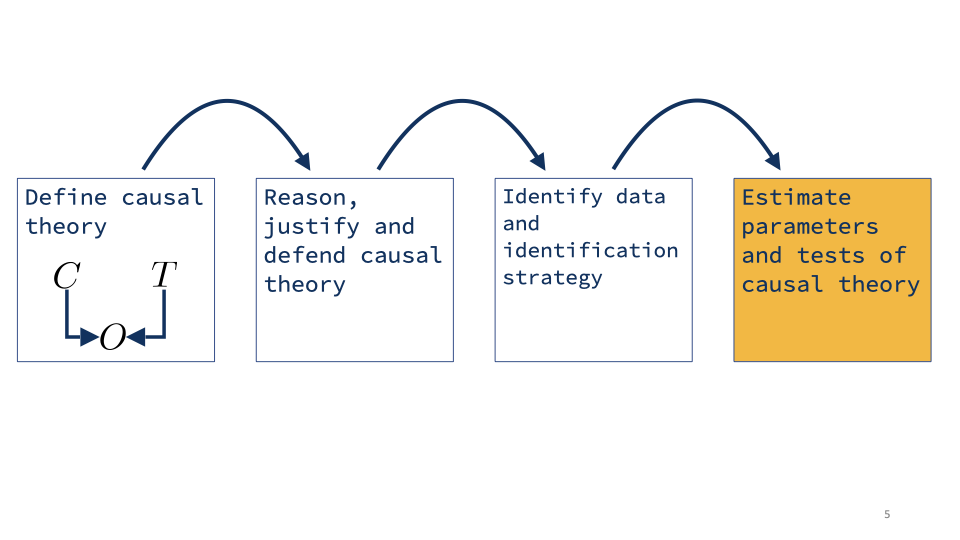
\includegraphics[width = \textwidth]{images/explanatory_workflow/explanatory_workflow_005.png}
\end{frame}

\begin{frame}
  \frametitle{How to Estimate Parameters}

  \begin{itemize}
  \item Estimate model and interpret coefficients
  \item Return to reasoning about the causal model and possible
    violations
  \end{itemize} 

   \note[item]{In explanatory analysis, like other points in the course
    to this point, the estimation is actually very straightforward.}
  \note[item]{For example, with experimental data, estimate an OLS.}
  \note[item]{However, it is the thinking, designing and interpreting
    that is both (a) important; and (b) hard.} 
 \note[item]{Standard errors which tell you about statistical
   uncertainty.  But what if your causal theory isn't quite right? We
   don't have an uncertainty measure on our theory.}
 \note[item]{At this point, you may have to think through
   possible ways it could be wrong.  This is a kind of sensitivity
   analysis.  If you think there might be an omitted causal pathway,
   for example, you'll try to think through how it would change your
   coefficients.  You may try to invent a way to correct for the
   problem, or run an additional analysis to provide evidence for
   whether it really is a problem.} 
\end{frame}


\begin{frame}
  \frametitle{The Explanatory Modeling Workflow}

  \note[item]{So there's the very high level view of what explanatory modeling is. }
  \note[item]{I hope that gives you some idea of how it's very
    distinct from what we've done before.  Explanatory modeling is its own specialized field. Now let's see some more
    details.} 

  \centering
  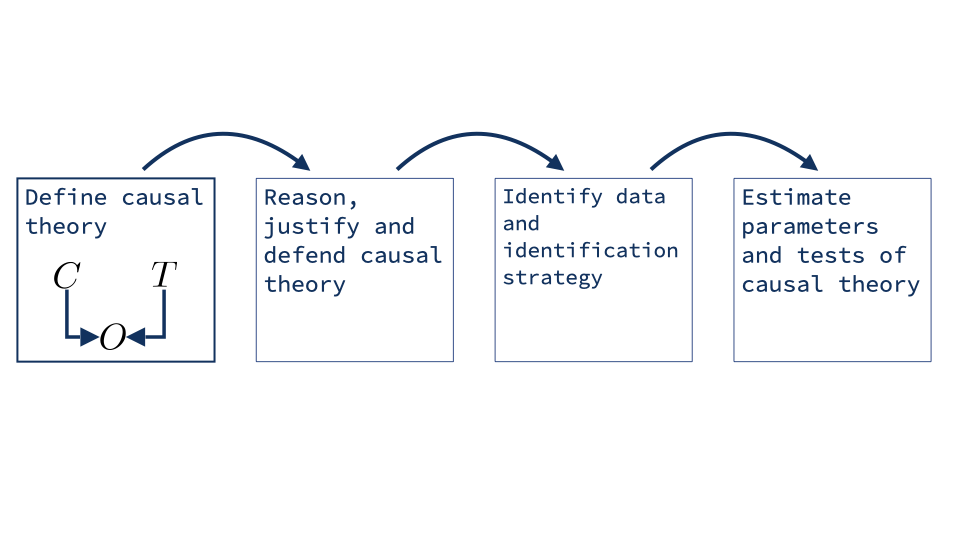
\includegraphics[width = \textwidth]{images/explanatory_workflow/explanatory_workflow_001.png}
\end{frame}

\begin{frame}
  \frametitle{WE SHOULD HAVE AN ACTIVITY HERE}
  \textbf{Note: We should either have a reading, or applied activity
    here.}
  \begin{itemize}
  \item Reading activity 
  \end{itemize}
\end{frame} 


\section{Pearl and Structural Equation Models}

\begin{frame}
  \frametitle{Toward a Flexible Causal Framework}
  \begin{columns}
    \begin{column}{0.6\textwidth}
      \centering
      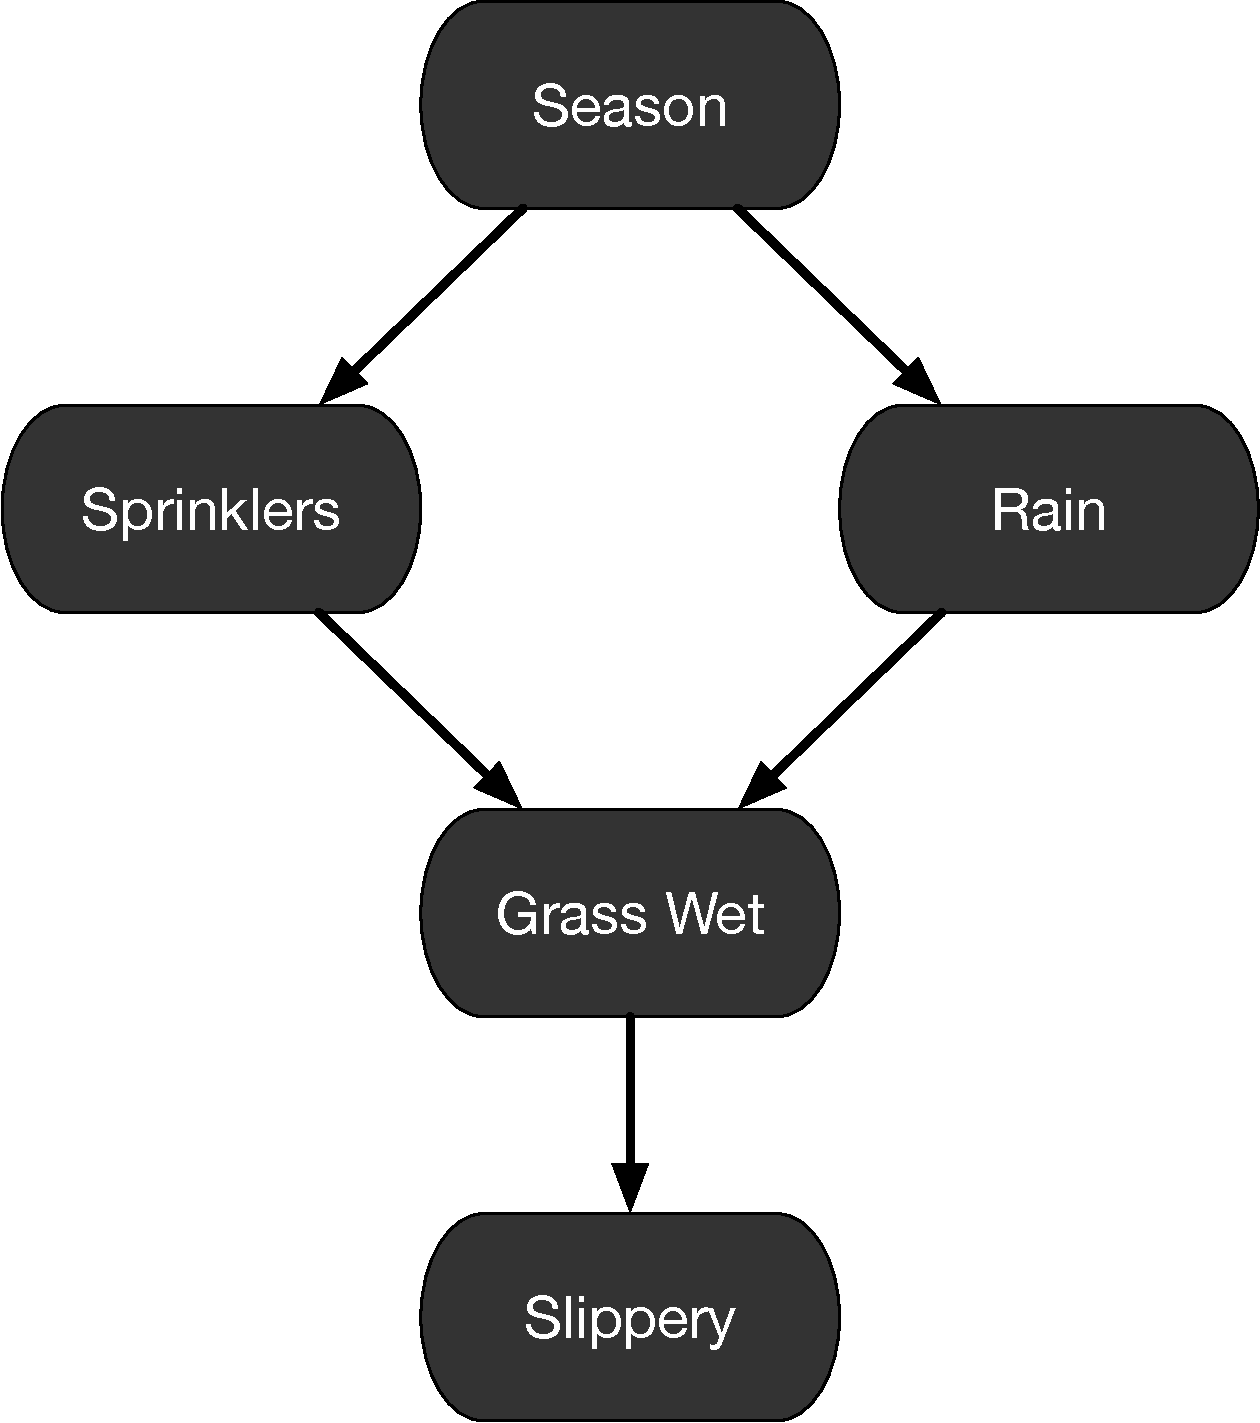
\includegraphics[width=.9\textwidth]{images/sprinklers}
      \textit{Causality} (2000, 2009)
    \end{column}
    \begin{column}{0.4\textwidth} 
      \centering
      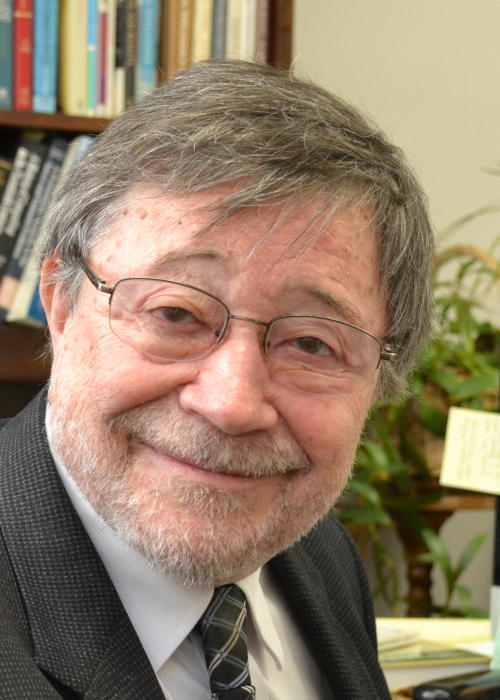
\includegraphics[width=\textwidth]{images/pearl}
      Judea Pearl 
    \end{column}
  \end{columns}
  \note[item]{I'm going to tell you about a specific line of
    causal models, which uses graphs to describe causal pathways.} 
  \note[item]{The core elements of this field were actually
    written by a computer scientist at UCLA, Judea Pearl. This is an
    ad-hominem attack, but he is \textit{definitely} causality's
    crazy grandpa.} 
  \note[item]{Judea Pearl was working at UCLA on expert systems
    and became interested in modeling causality as a tool for
    machines to make decisions or to understand the world.}
  \note[item]{This would normally be considered an advanced topic.
    We chose this as a starting point we want to equip you to
    recognize all the causal assumptions 
    that go into an analysis --  we don't want some of those
    assumptions to be hidden or implicit.}
  \note[item]{This mode of reasoning will give us a visual way to
    make our assumptions very explicit.}
  \note[item]{However, and we will cover this at the end of this
    section, we never get to directly \textit{see} the causal graph; a
    fundamental, and insurmountable limitation.} 
\end{frame}

\begin{frame}
  \frametitle{How to Reason About a Causal Theory}
  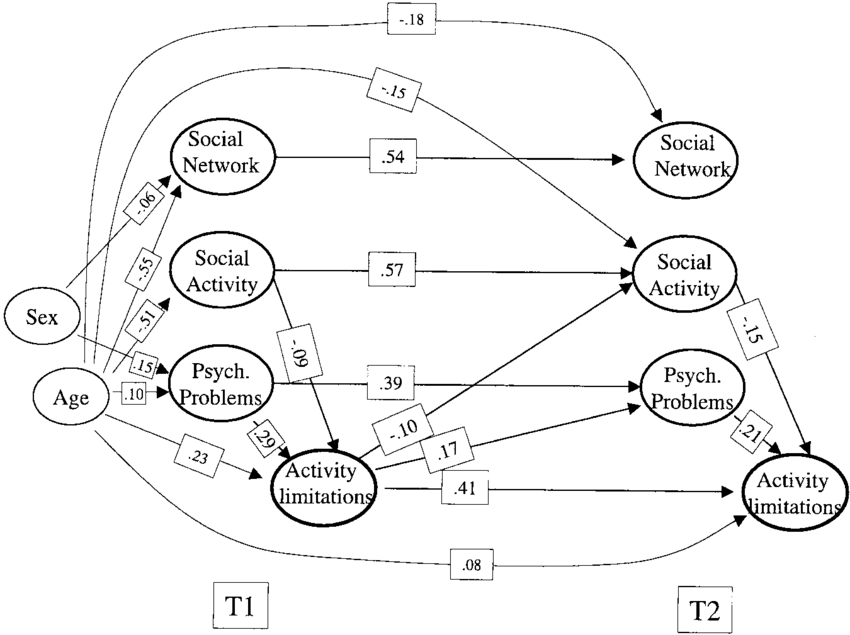
\includegraphics[width=\textwidth]{images/psych_structural_model}
  \note[item]{If there are no limitations on your causal graph,
    incredible complexity is possible.}
  \note[item]{This graph contains only two sets of variables -- one
    set  of``controls'' (age, sex), and another set of confounders.
    Data is measured through time, so some are
    repeated; and the authors have estimated relationships through
    time.}
  \note[item]{The point that we want to bring home here is that
    without structure, these quickly reflect the complexity of of the
    world.} 
\end{frame}


\begin{frame}
  \frametitle{Structural Equation Model (SEM) Basics}
   
  \begin{columns}
    \begin{column}{0.6\textwidth}
      \textbf{Endogenous variables}
      \begin{itemize}
      \item $V$: Vaccine
      \item $A$: Antibodies
      \item $I$: Infection
      \end{itemize}

      \textbf{Background variables}
      \begin{itemize}
      \item $\epsilon$: Outside causes
      % \item Often hidden
      \end{itemize}
   
      \textbf{Structural equations}
      \begin{itemize}
      \item $V = f_V(\epsilon_1)$
      \item $A = f_A(V, \epsilon_2)$
      \item $I = f_I(A, \epsilon_3)$
      \end{itemize}      
    \end{column}

    \begin{column}{0.4\textwidth}
      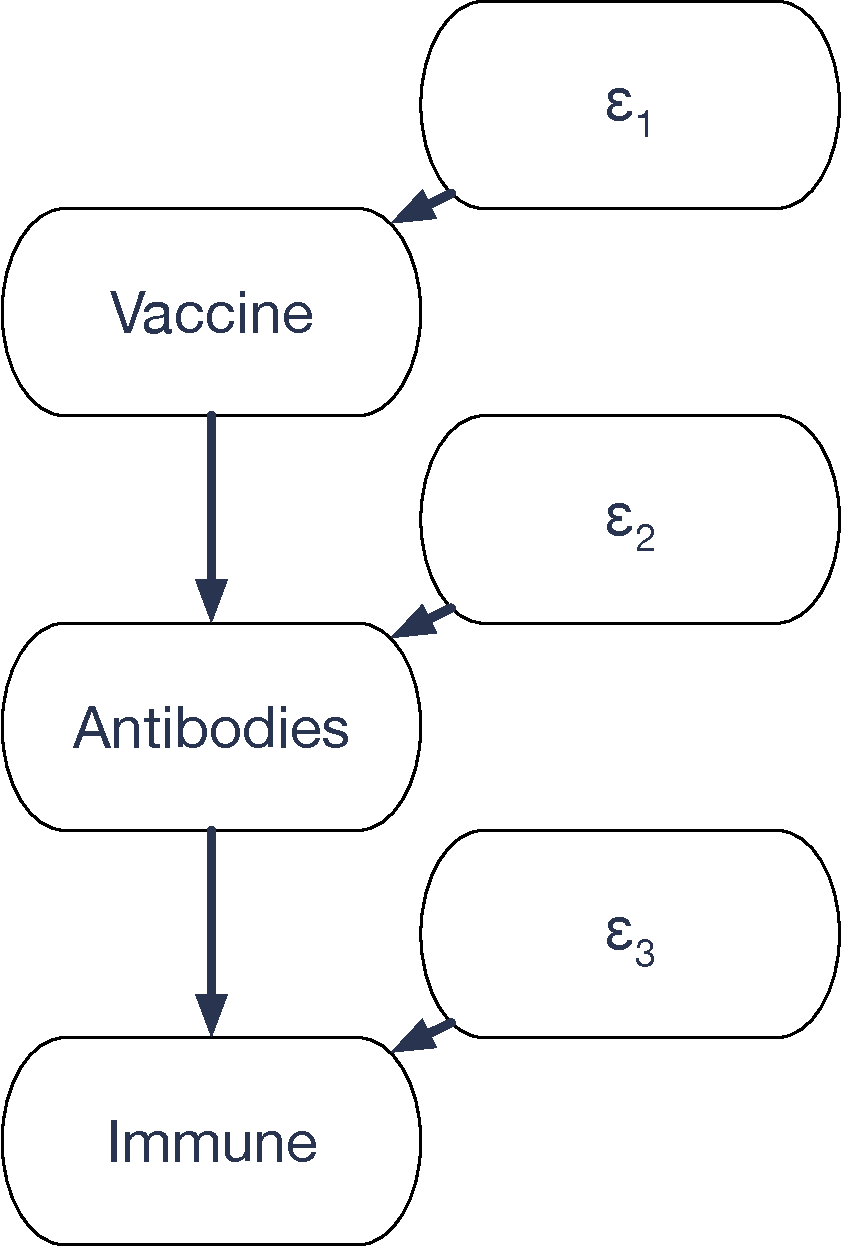
\includegraphics[width=\textwidth]{images/vaccine_graph}
    \end{column}
  \end{columns}

  \note[item]{\alex{Lets flip this graph.}}
  \note[item]{\alex{Let's also include $\epsilon$}}
  \note[item]{Here's what one of these models might look like} 
  \note[item]{Suppose that we focus on a subset of the variables on
    the directed graph. Each link is a causal effect} 
  \note[item]{For discussion we can think of two types of variables --
    those that are in focus, and those that we're ``blurring'' out --
    but in fact, they're all the same. Those that are \textit{in
      focus} we might call the endogenous variables, determined within
    the model. There is also set of background variables All of 
    the randomness comes from the background variables. They
    represent causes that come from outside the system.} 
  \note[item]{Finally, we have the structural equations.  These
    tell us how each endogenous variable responds to its parents
    in the causal graph} 
  \note[item]{For example, $A$ has two parents: $V$ and
    $\epsilon_2$.  So the structural equation for $A$ says that
    its value will be a function of $V$ and $\epsilon_2$.} 
  \note[item]{These functions encode what we call counterfactuals.
    Each patient either has the vaccine or does not have the
    vaccine.  But the function $f_A$ represents what would have
    happened under either state.} 
\end{frame}

\subsection{Reading: Alleged Dangers of Cigarette Smoking} 

\begin{frame}
  \frametitle{Reading: Alleged Dangers of Cigarette Smoking}
  \textbf{Note: This is a reading call. We're just placing it here for
    organization.}

  \begin{columns}
    \column{.7\linewidth}
    Read the two-page article, published in the BMJ in 1957 written by
    Ronald A. Fisher. Some context. R.A. Fisher is
    
    \begin{itemize}
    \item Perhaps the most influential statistician \textit{of all time}
    \item At the very least, up there with Bayes, Neyman, and the
      canon. 
    \item The student interested in a longer-form profile of this
      content can read the following article written by Pricenomics.
      \href{https://priceonomics.com/why-the-father-of-modern-statistics-didnt-believe/}{[Link
        here]}.
    \end{itemize}
    
    \column{.3\linewidth}
    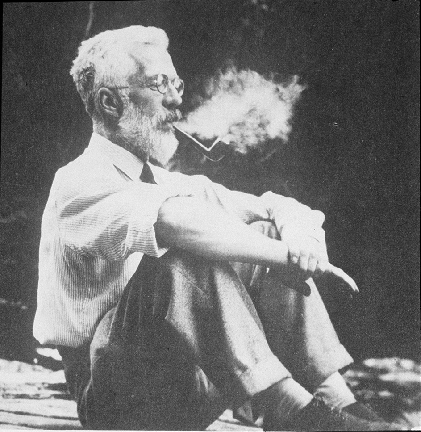
\includegraphics[width=\textwidth]{images/fisher.png}
    Of course, smoking causes lung cancer -- Fisher was dogmatic.
  \end{columns}
\end{frame}

\subsection{Evaluation and Execution of a Structural Equation Model} 

\begin{frame}
  \frametitle{Example: Execution of an SEM}
  \textbf{Note: This is a whiteboard, we're just placing it here for
    organization.}
  \begin{itemize}
  \item What causes lung cancer? 
  \item Coffee $\rightarrow$ Alertness $\rightarrow$ Work 
  \item Interest $\rightarrow$ Awareness $\rightarrow$ Purchase
  \end{itemize} 
\end{frame}

\begin{frame}
  \frametitle{}
\end{frame} 

\begin{frame}
  \frametitle{Execution of an SEM}
  
  \begin{columns}
    \begin{column}{0.6\textwidth}
      
      \textbf{Step one}
      \begin{itemize}
      \item Draw values of $\epsilon_1, \epsilon_2, \epsilon_3$.
      \item Assume $\epsilon_{1} \dots \epsilon_{k}$ are independent
      \end{itemize} 
    
      \textbf{Step two}
      \begin{itemize}
      \item Assign endogenous variables their values
      \end{itemize} 
      
      \begin{align*}
        V &= f_V(\epsilon_1) \\ 
        A &= f_A(V, \epsilon_2) \\ 
        I &= F_I(A, \epsilon_3) \\
      \end{align*}
      
      % \vspace{1cm}
      % \footnotesize{Note: If there are cycles, we assume the
      % equations have a unique solution} 
      \note[item]{There's a lot more to Pearl's theory, but there you
        can see just the basic idea of an SEM.} 
      
    \end{column}
    \begin{column}{0.4\textwidth}
      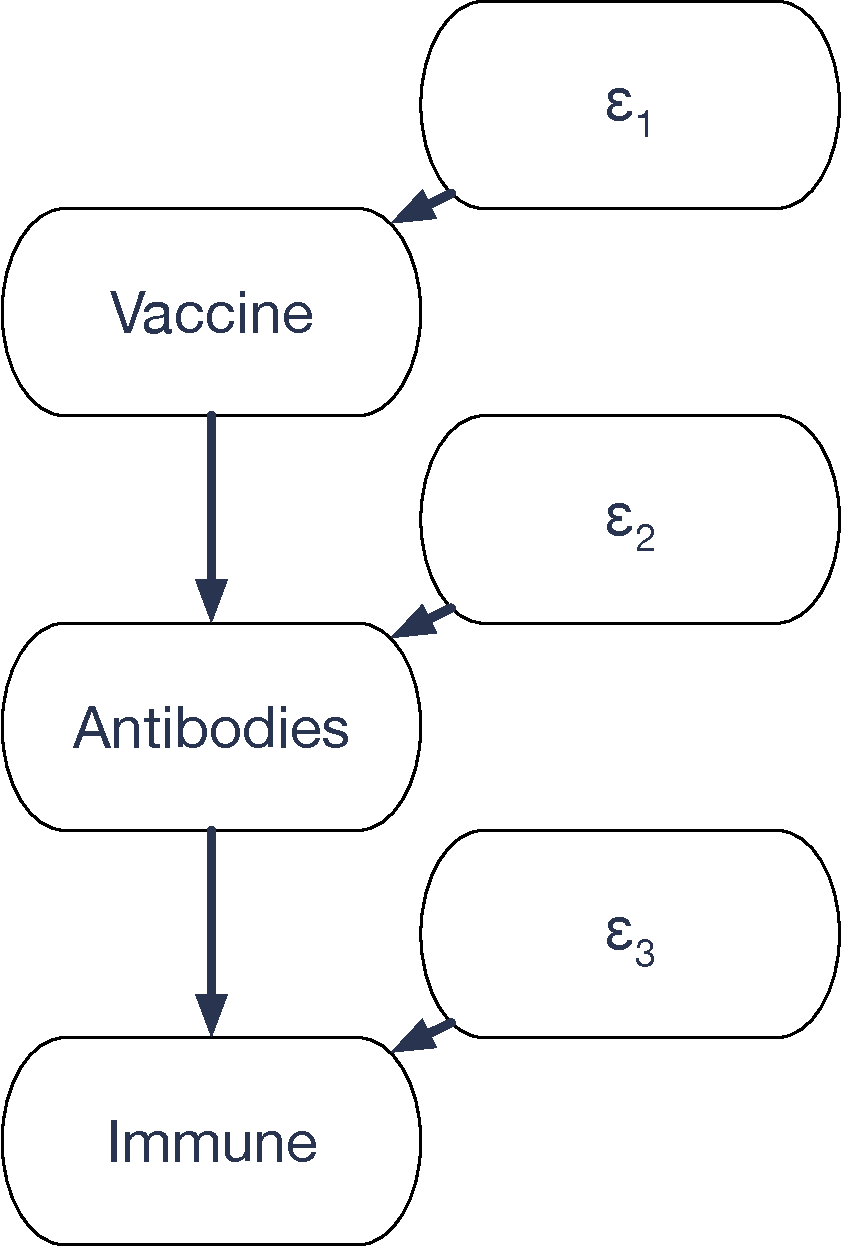
\includegraphics[width=\textwidth]{images/vaccine_graph}
      
    \end{column}
  \end{columns}
  \note[item]{How do the variables in an SEM get their values?}  
  \note[item]{First step, the background variables have their values
    drawn.} 
  \note[item]{Next, we have to follow the causal pathways and see what 
    values each of the endogenous variables gets. Here, we can start
    with V...} 
\end{frame}

% \section{Learnosity Check}

% \begin{frame}
%   \frametitle{Executing An SEM}

%   \begin{columns}
%     \begin{column}{0.6\textwidth}

%       In this SEM, assume the following:

%       $\epsilon_1, \epsilon_2, \epsilon_3$ are Bernoulli variables.
%       \begin{itemize}
%       \item $P(\epsilon_1 = 1) = 2/3$
%       \item $P(\epsilon_2 = 1) = 3/4$
%       \item $P(\epsilon_3 = 1) = 1/2$

%       \item $V = f_V(\epsilon_1) = \epsilon_1$
%       \item $A = f_A(V, \epsilon_2) = V \cdot \epsilon_2$
%       \item $I = f_I(A, \epsilon_3) = (1-A) \cdot \epsilon_3$
%       \end{itemize}
%       What is $P(I=1)$, representing an infection?
%       \paul{(Answer: 1/4)}

%     \end{column}
%     \begin{column}{0.4\textwidth}
%       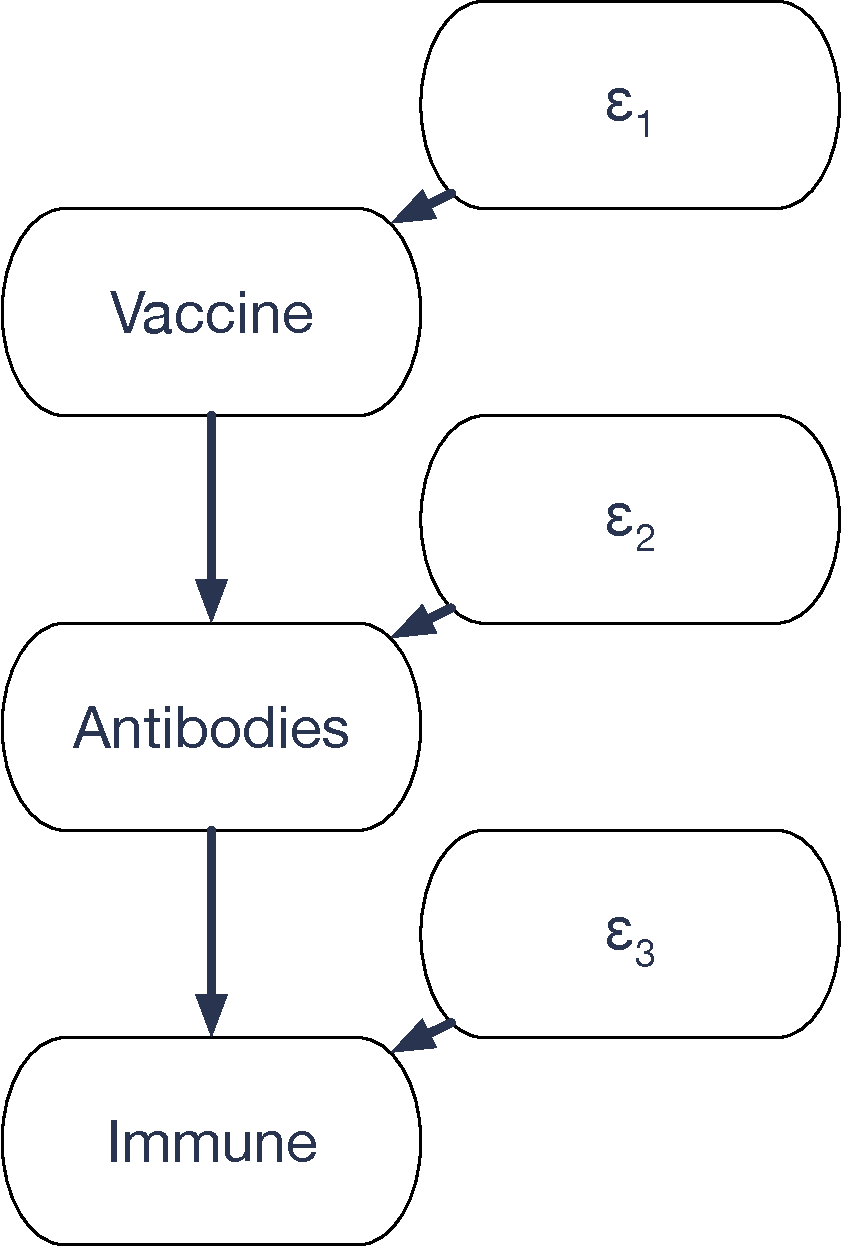
\includegraphics[width=\textwidth]{images/vaccine_graph}
%     \end{column}
%   \end{columns}
% \end{frame}

\section{Statistical Implications of a Causal Graph}

\begin{frame}
  \frametitle{How to Apply an SEM}
  
  % 1. Choose functional forms, fit to data

  % \begin{itemize}
  % \item Used in some areas (e.g. supply and demand)
  % \item Overall, not common.
  %   \begin{itemize}
  %   \item How do you justify the functions you choose?
  %   \end{itemize}
    
  % \end{itemize}
  
  Causal models require that we write down, clearly, the assumptions
  about the causal process \textit{in the data generating process}.
  \begin{itemize}
    \item Evaluate how closely our data matches our \textit{theory}
      about the world
    \item Choose an appropriate estimator for the data and theory 
  \end{itemize}
  % \paul{Currently, this slide doesn't seem to motivate causal graphs?}
  
  % \begin{itemize}
  % \item No need to specify functional forms
  % \end{itemize}
  
  \note[item]{Now you know a little bit about SEMS, but how do you
    apply them?} 
  \note[item]{One idea is to choose functional forms for each
    structural equation, then fit to data to estimate parameters.  } 
  \note[item]{This is actually done in some areas.  One classic
    example is estimating supply curves and demand curves.} 
  \note[item]{But on the whole, these type of models aren't very
    common.  And the reason is that they are so highly specified.  How
    can you convince somebody that the functions you chose are
    accurate depictions of reality?} 
  \note[item]{There's another approach though, which is to use the
    causal graph to derive statistical assumptions.  So it doesn't
    matter what the functions are!  we just need to make sure we get
    the graph right.} 
\end{frame}

\begin{frame}
  \frametitle{Causal Graph Definition}

  \begin{block}{Causal graph}
    A \textbf{causal graph} is a graph that describes the causal
    pathways among a subset of all variables.
  \end{block}

  Causal graphs encode our theory about the causal structure: 
  
  \note[item]{I put in the word subset, which means that we normally
    don't put in background variables, and we don't have to put in
    every possible variable in the world.  But there are two rules:} 

  \begin{enumerate}
  \item If there is an arrow from $X$ to $Y$, then $X$ has a direct
    causal effect on $Y$. 
  \item If there is \textbf{no} arrow from $X$ to $Y$, $X$ has
    \textbf{no} direct causal effect on $Y$. 
  \item If $X$ and $Y$ have a common cause $Z$, then $Z$ must be in
    the diagram, even if we cannot measure it.
  \end{enumerate}
  \note[item]{This last condition -- that it go in the diagram even if
    we cannot measure it is a fail-safe that keeps us from being lazy,
    or missing connections that we should be worried about.} 
\end{frame}
  
\begin{frame}
  \frametitle{Examples of Causal Graphs}
  \begin{block}{Example: Direct and indirect effects}
    \begin{itemize}
    \item $V \rightarrow A \rightarrow I$.  Vaccines have a direct
      causal effect on Antibodies, but no direct effect on
      Infection. 
    \end{itemize}    
  \end{block}
  \vspace{1em}
  \begin{block}{Example: Common Causes}
    \begin{itemize}
    \item Education $\rightarrow$ Wage.  Do we need to include motivation?
    \end{itemize}
  \end{block} 
\end{frame}


\begin{frame}
  \frametitle{Statistical Implications of a Causal Graph}
 
 \note[item]{A causal graph is a causal model, but it has statistical 
   implications.} 

 \begin{block}{Theorem: independence} 
   If $X$ and $Y$ have no common ancestors in an
   acyclic SEM, they are independent.
 \end{block} 
 
 \begin{columns}
   \begin{column}{0.7\textwidth}  
   \note[item]{\paul{worried this is too much to write}}
     \note[item]{If $X$ and $Y$ are background variables, true by
       assumption.} 
     \note[item]{Induction: Assume the statement is true for all $X$
       and $Y$ in a set $S$, and let $Z$ be any node whose parents,
       labeled $P_1,P_2,...,P_k$ are all in $S$.  If $X \in S$ and $X$
       and $Z$ have no common causes, then $X$ shares no common causes
       with each $P_i$...} 
     \note[item]{Let's draw a set S on this graph}
     \note[item]{How would you finish this proof?  $\implies X \indep
       P_i$.  Therefore, $X \indep Z = f_Z(P_1,P_2,...,P_k)$, and the
       statement is true for all $X$ and $Y$ in $S \cup \{Z\}$.}      
   \end{column}
   
   \begin{column}{0.4\textwidth}
     \vspace{2em}
     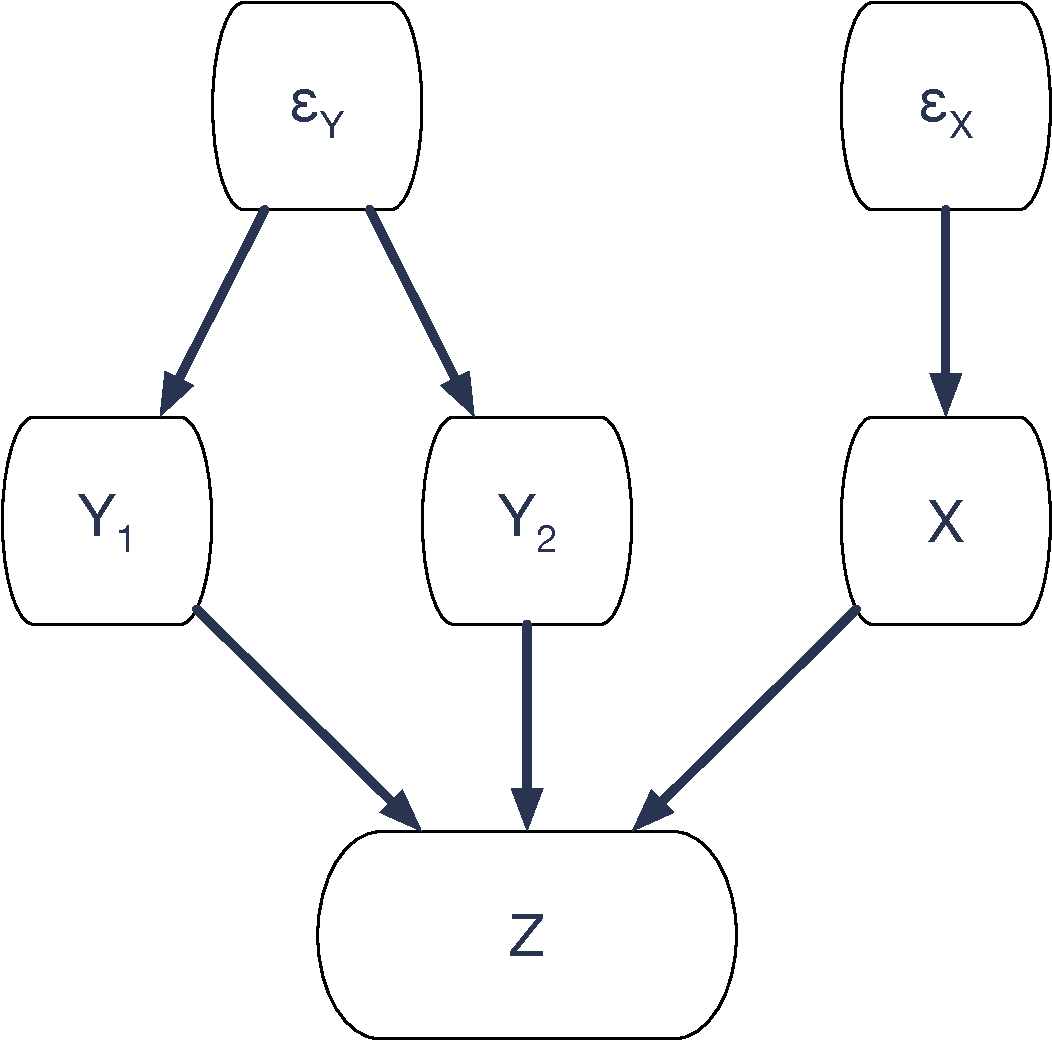
\includegraphics[width=\textwidth]{images/independence_graph}
   \end{column}
 \end{columns}
 \vspace{2cm}
 % \footnotesize Note: Can be extended to cyclic graphs with extra
 % conditions. 
 
 \note[item]{What is this telling us? In an SEM, associations don't
   happen by accident.  The reason that variables are dependent is
   because of common causes.  The randomness in $X$ and $Y$ come from
   background variables.  If they don't share any of the same
   background variables as ancestors, they must be independent} 
 
\end{frame}

% \section{Learnosity Check}

% \begin{frame}
%   \frametitle{Independence in Causal Graphs}
%   \textbf{Note: This is a learnosity activity. We're placing it here
%     for organization.}

%   \begin{columns}
%     \column{0.7\linewidth}
%     In this causal graph, which pairs of variables are independent?
%     \centering
%     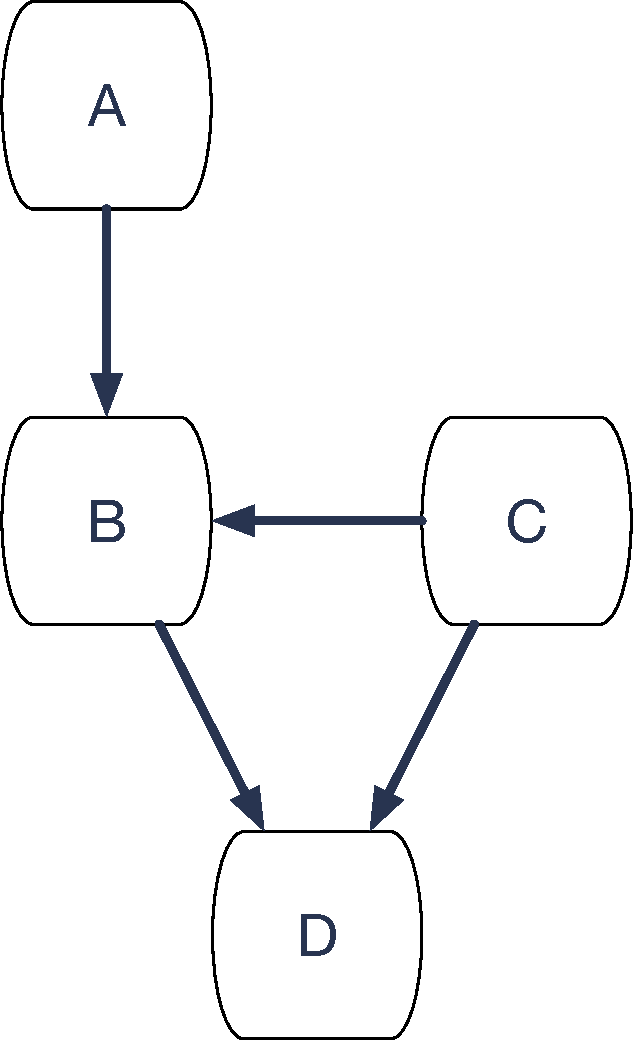
\includegraphics[width=.3\textwidth]{images/dag_check_1}
%     \column{0.3\linewidth}
%     \paul{Answer: A and D}
%   \end{columns}
%   \note[item]{\alex{This is great -- let's make more to get students
%       into the flow of these!}}
% \end{frame}

\section{The One-Equation Structural Model}

\begin{frame}
  \frametitle{The Simplest Causal Graph}
  
  \note[item]{Let's take a look at the simplest possible causal graph.
    A lot of econometrics textbooks start off like this, but without
    making the assumptions explicit.} 
  
  One causal relationship:
  
  \begin{itemize}
  \item A single outcome: $Max\_Speed$
  \item A set of background variables that have a causal effect on the
    outcome: $HP$, $Weight$ 
  \item An error term that also has a causal effect on the outcome:
    $\epsilon$ 
  \end{itemize}
  \note[item]{We'll say more about the error term in just a moment.}   
\end{frame}

\begin{frame}
  \frametitle{The One-Equation Structural Model}
  
  \note[item]{We can express this theory as a causal graph.  The only
    arrows are from the inputs to the outcome.} 
  
  \centering
  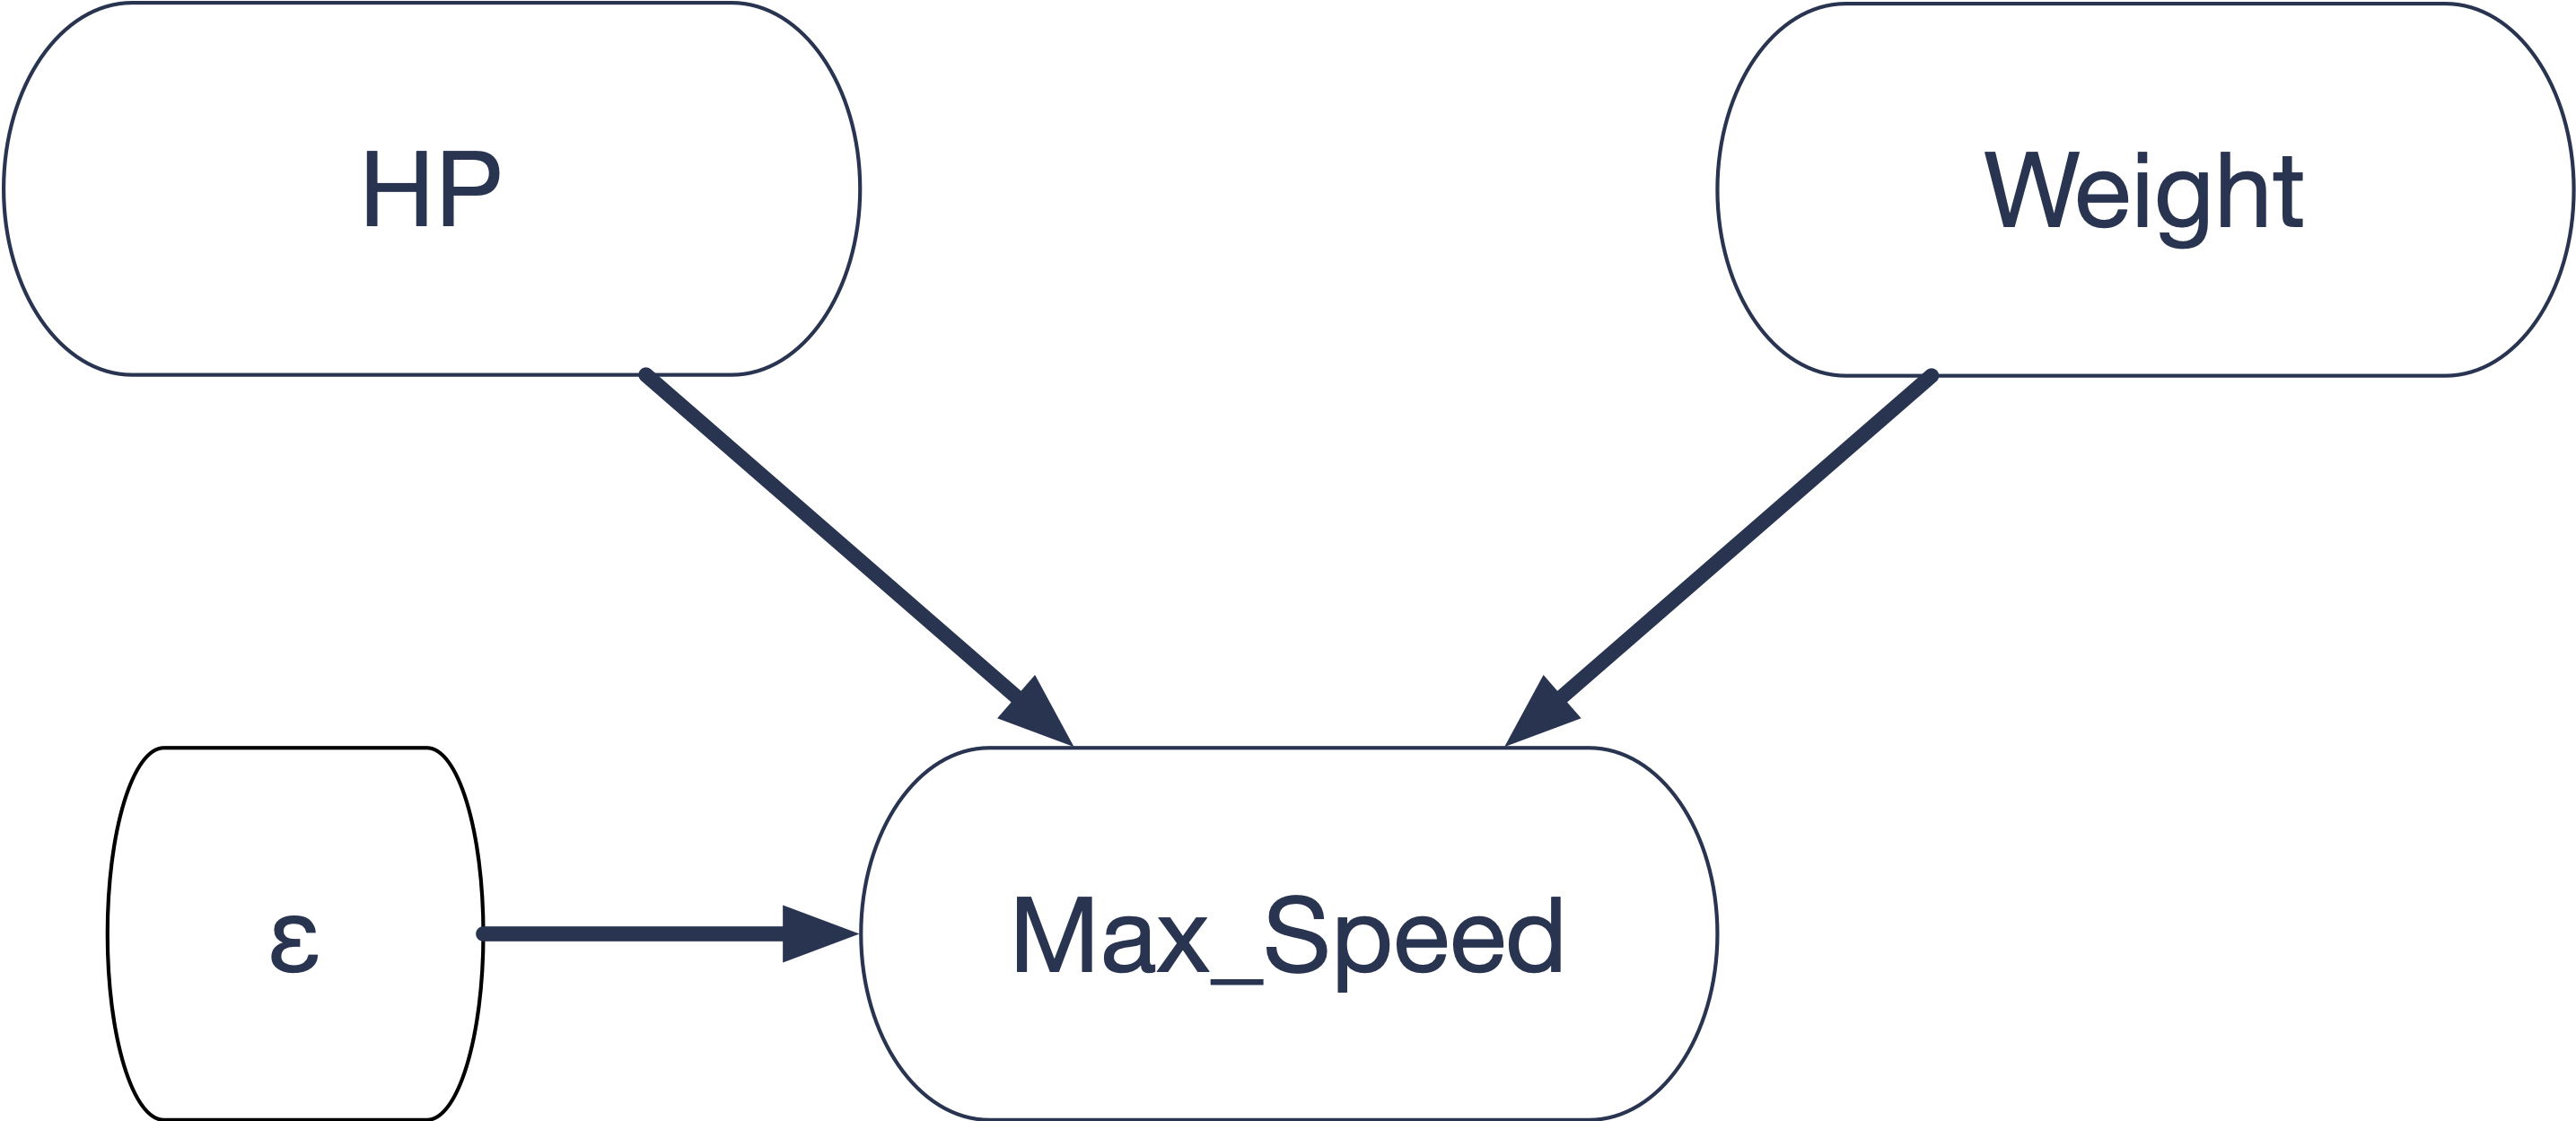
\includegraphics[width = .6\textwidth]{images/causal_graph_base}
  
  \note[item]{If we assume the relationship is linear, we can also
    express it as a structural equation.} 
  
  \begin{align*}
    Max\_Speed  &= \beta_0 + \beta_1 HP + \beta_2  Weight + \epsilon
                  \tag{S} \\
    \text{Where } E[\epsilon] &= 0
  \end{align*}
  
  \note[item]{This might look like any other linear equation, but it's
    not.  We're inside a causal model, and we're saying this equation
    represents the response of max speed to the inputs.} 
  \note[item]{If you put in different values of HP and Weight, you get
    a different max speed as a result.  That's what the causal model
    says} 
  \note[item]{We'll place an S next to structural equations to make
    them clear.} 
  \note[item]{Now if I manipulate this equation - say I solve for HP -
    it's still a valid equality, but it stops holding any causal
    interpretation.} 
\end{frame}



\begin{frame}
  \frametitle{The Error Term in Structural Equations}
  
  \note[item]{While we were doing pure statistics, we had an error
    term, and it represented the difference between our prediction and
    the target.  It had no special meaning beyond that.} 
  
  \textbf{To a statistician:} $\epsilon$ is the difference between the
  target and the prediction 
  
  \textbf{To an explanatory modeler:} $\epsilon$ is unmeasured factors
  that have a causal effect on the outcome
  
  \note[item]{But that's not how econometricians, or political
    scientists, or epidemiologists look at $\epsilon$. } 
  \note[item]{To them $\epsilon$ is another random variable in a
    causal model.  It represents factors in the real world, but ones
    that we can't measure.} 
\end{frame}

\begin{frame}
  \frametitle{The Error Term in Structural Equations (cont.)}
  \note[item]{Think about the car.  We know that HP and Weight aren't
    the only things that make a car faster or slower.  That's why HP
    and Weight don't predict speed perfectly with zero error.} 
  \note[item]{Choose some other factor and write it down.  If you
    still can't predict speed perfectly, choose yet another factor and
    write it down.  Keep going an infinite number of times if you have
    to.} 
  
  \textbf{Thought experiment:} Write down any missing variable that
  can affect the outcome. 
  
  \begin{align*}
    Max\_Speed  = &\beta_0 + \beta_1 HP + \beta_2  Weight \\
                  &+ \underbrace{\beta_3 Air\_Resistance + \beta_4 Tires + ...}_{\mathlarger{\mathlarger{\epsilon}}}
  \end{align*}
  % \hspace{3cm} 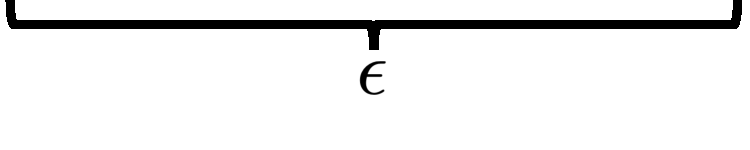
\includegraphics[width =
  % .63\textwidth]{images/epsilon}
  
  \note[item]{If we could actually write down every possible factor
    that affects the outcome, maybe there would be no error left.} 
  \note[item]{However, we can't possibly measure all of these factors.
    So we write down $\epsilon$ to represent them.} 
  \note[item]{What does this mean?  We can't just assume the error
    term behaves the way we want.  we have to think about what factors
    might be inside it, and where they actually go in the causal
    graph.} 
\end{frame}

\begin{frame}[t]
  \frametitle{Assessing the Causal Graph}
  
  \vspace{.5cm}
  \begin{center}
  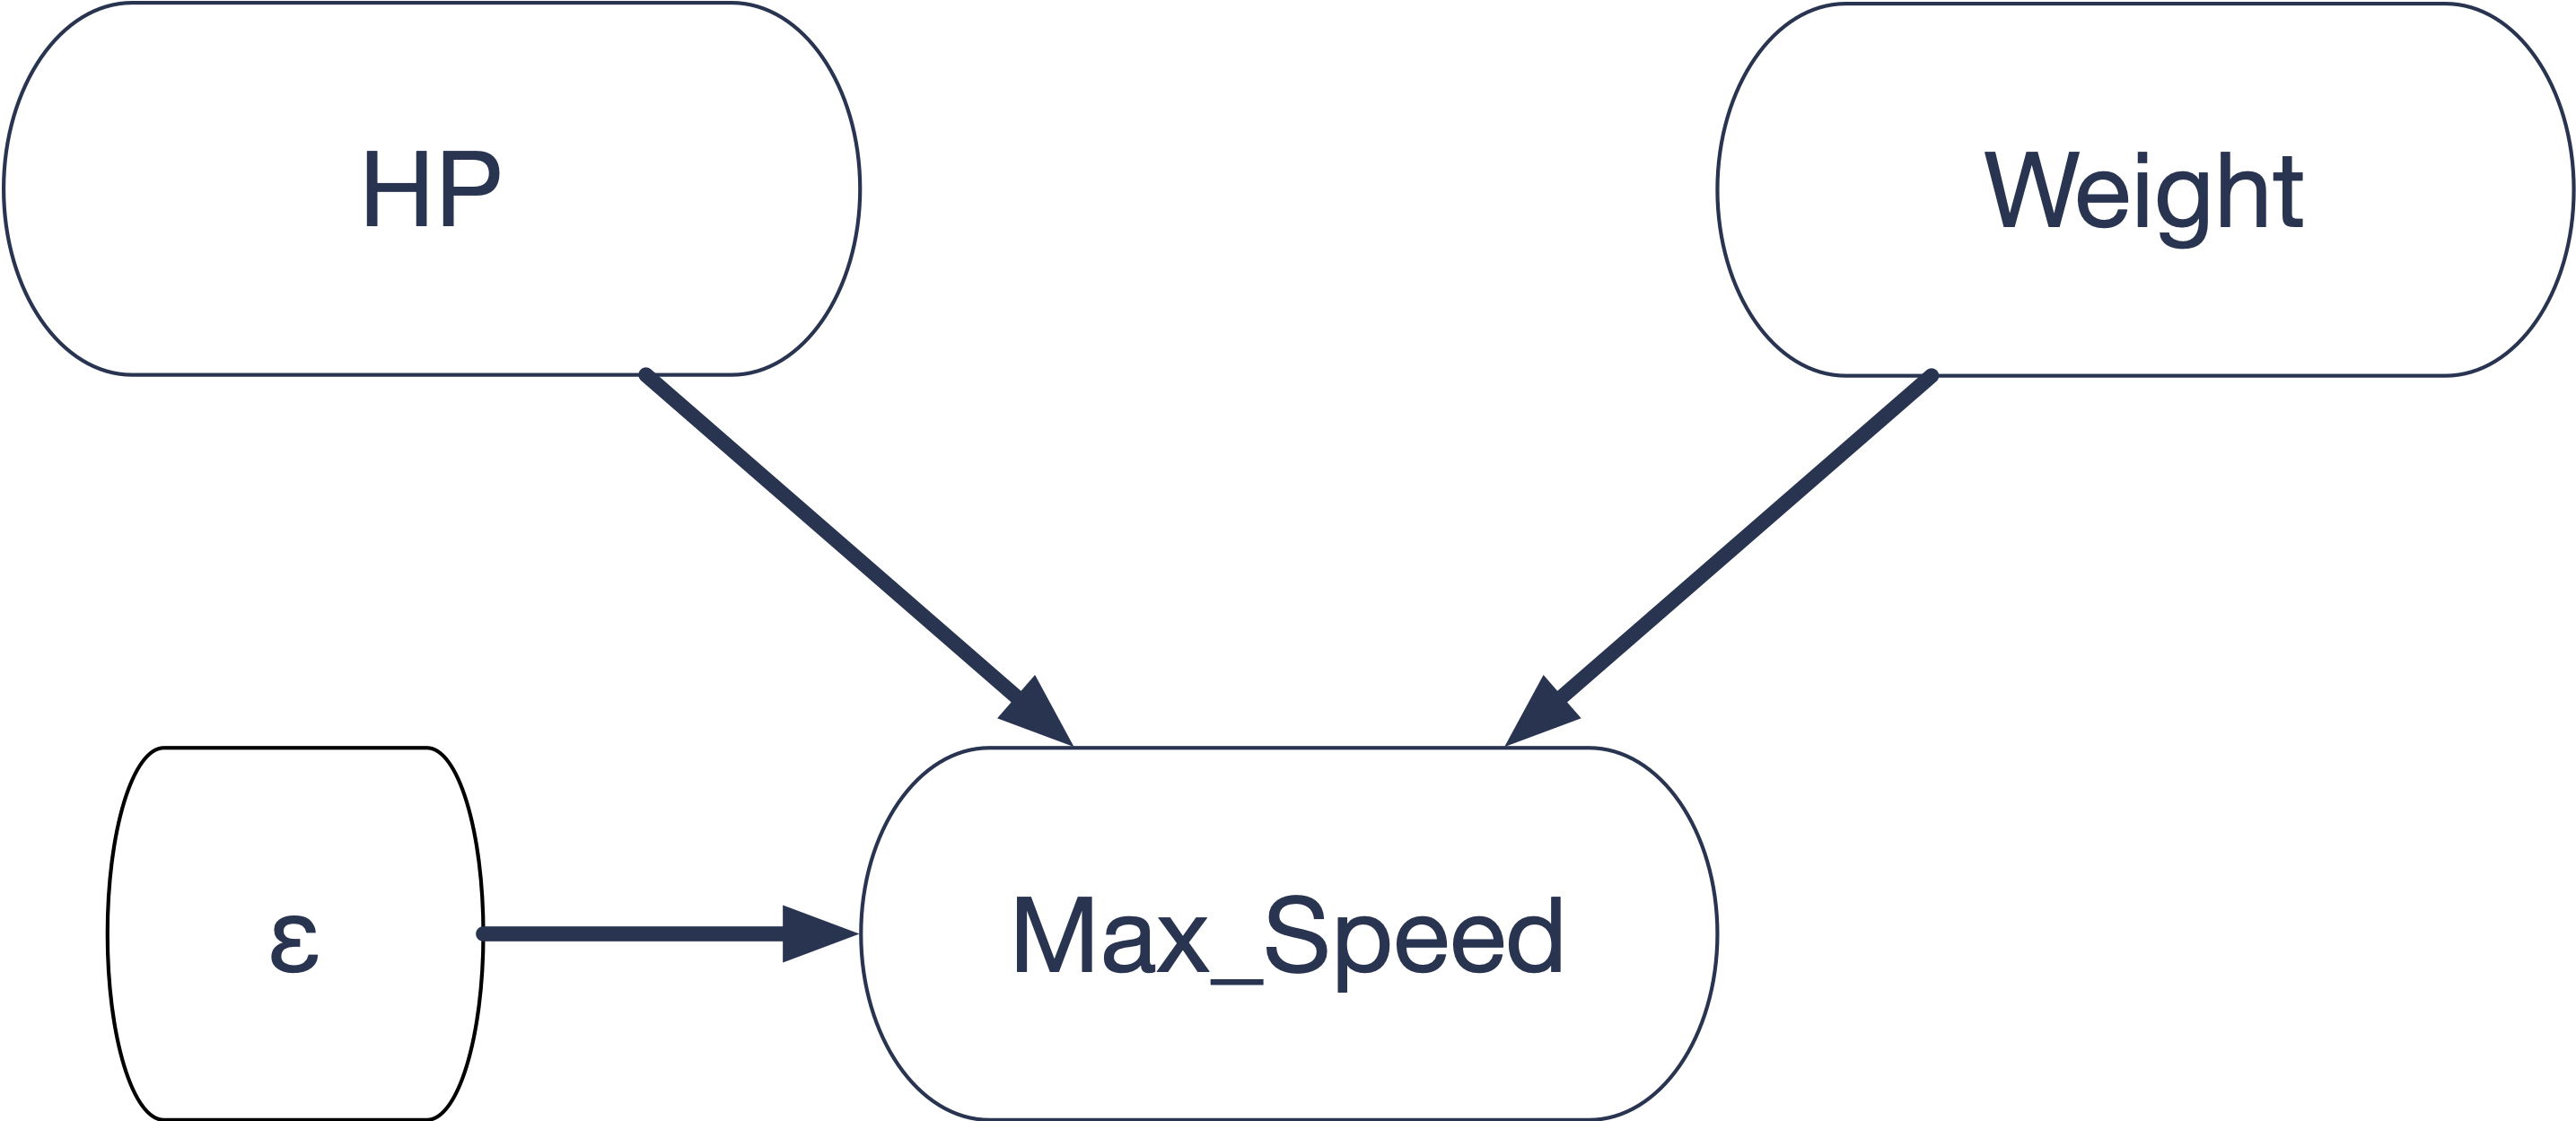
\includegraphics[width = .6\textwidth]{images/causal_graph_base}
  \end{center}
  
  \note[item]{Here's what our causal graph looks like again.  Now
    let's think about exactly what we're assuming here. Remember we
    have two rules. } 
  \note[item]{First, if there's no arrow somewhere, there's no direct
    effect. So in particular, we're assuming that there's no path from
    Max speed back to HP} 
  \note[item]{And if there was any common cause of HP and Max speed,
    we would have to add it.  What if we were wrong about air
    resistance,  we thought it only had an effect on max speed, but
    what if it also has an effect on HP?  We're assuming there's no
    variable like that.} 
  \note[item]{\paul{Now you might wonder, did we get the top of the
      graph right?  It's generally ok if HP and Weight have a common
      cause up here.  Or even if they cause each other, which we'll
      discuss later.  But no more arrows involving Max Speed! }} 
  
  Two things we look for:
  \begin{enumerate}
    \item Are there any causal pathways back from $Max\_Speed$ to $HP$ and $Weight$?
    \item Are there any common ancestors of $HP$ and $Max\_Speed$ or
      of $Weight$ and $Max\_Speed$?
    \end{enumerate} 
  
  \note[item]{If we believe that this graph is valid, that's really good news for estimation.}
  
\end{frame}



\begin{frame}[t]
  \frametitle{Estimation in the One-Equation Model}
  
  \note[item]{Ok, we've done all this work, so that we can write down
    exactly what the one-equation structural model is.} 
  \note[item]{Now we're ready to estimate its coefficients.  and the
    way we do that is with OLS regression.} 
  \note[item]{The proof that OLS works is really quick with all the
    machinery we've built...} 
  
  \vspace{.5cm}
  \begin{center}
  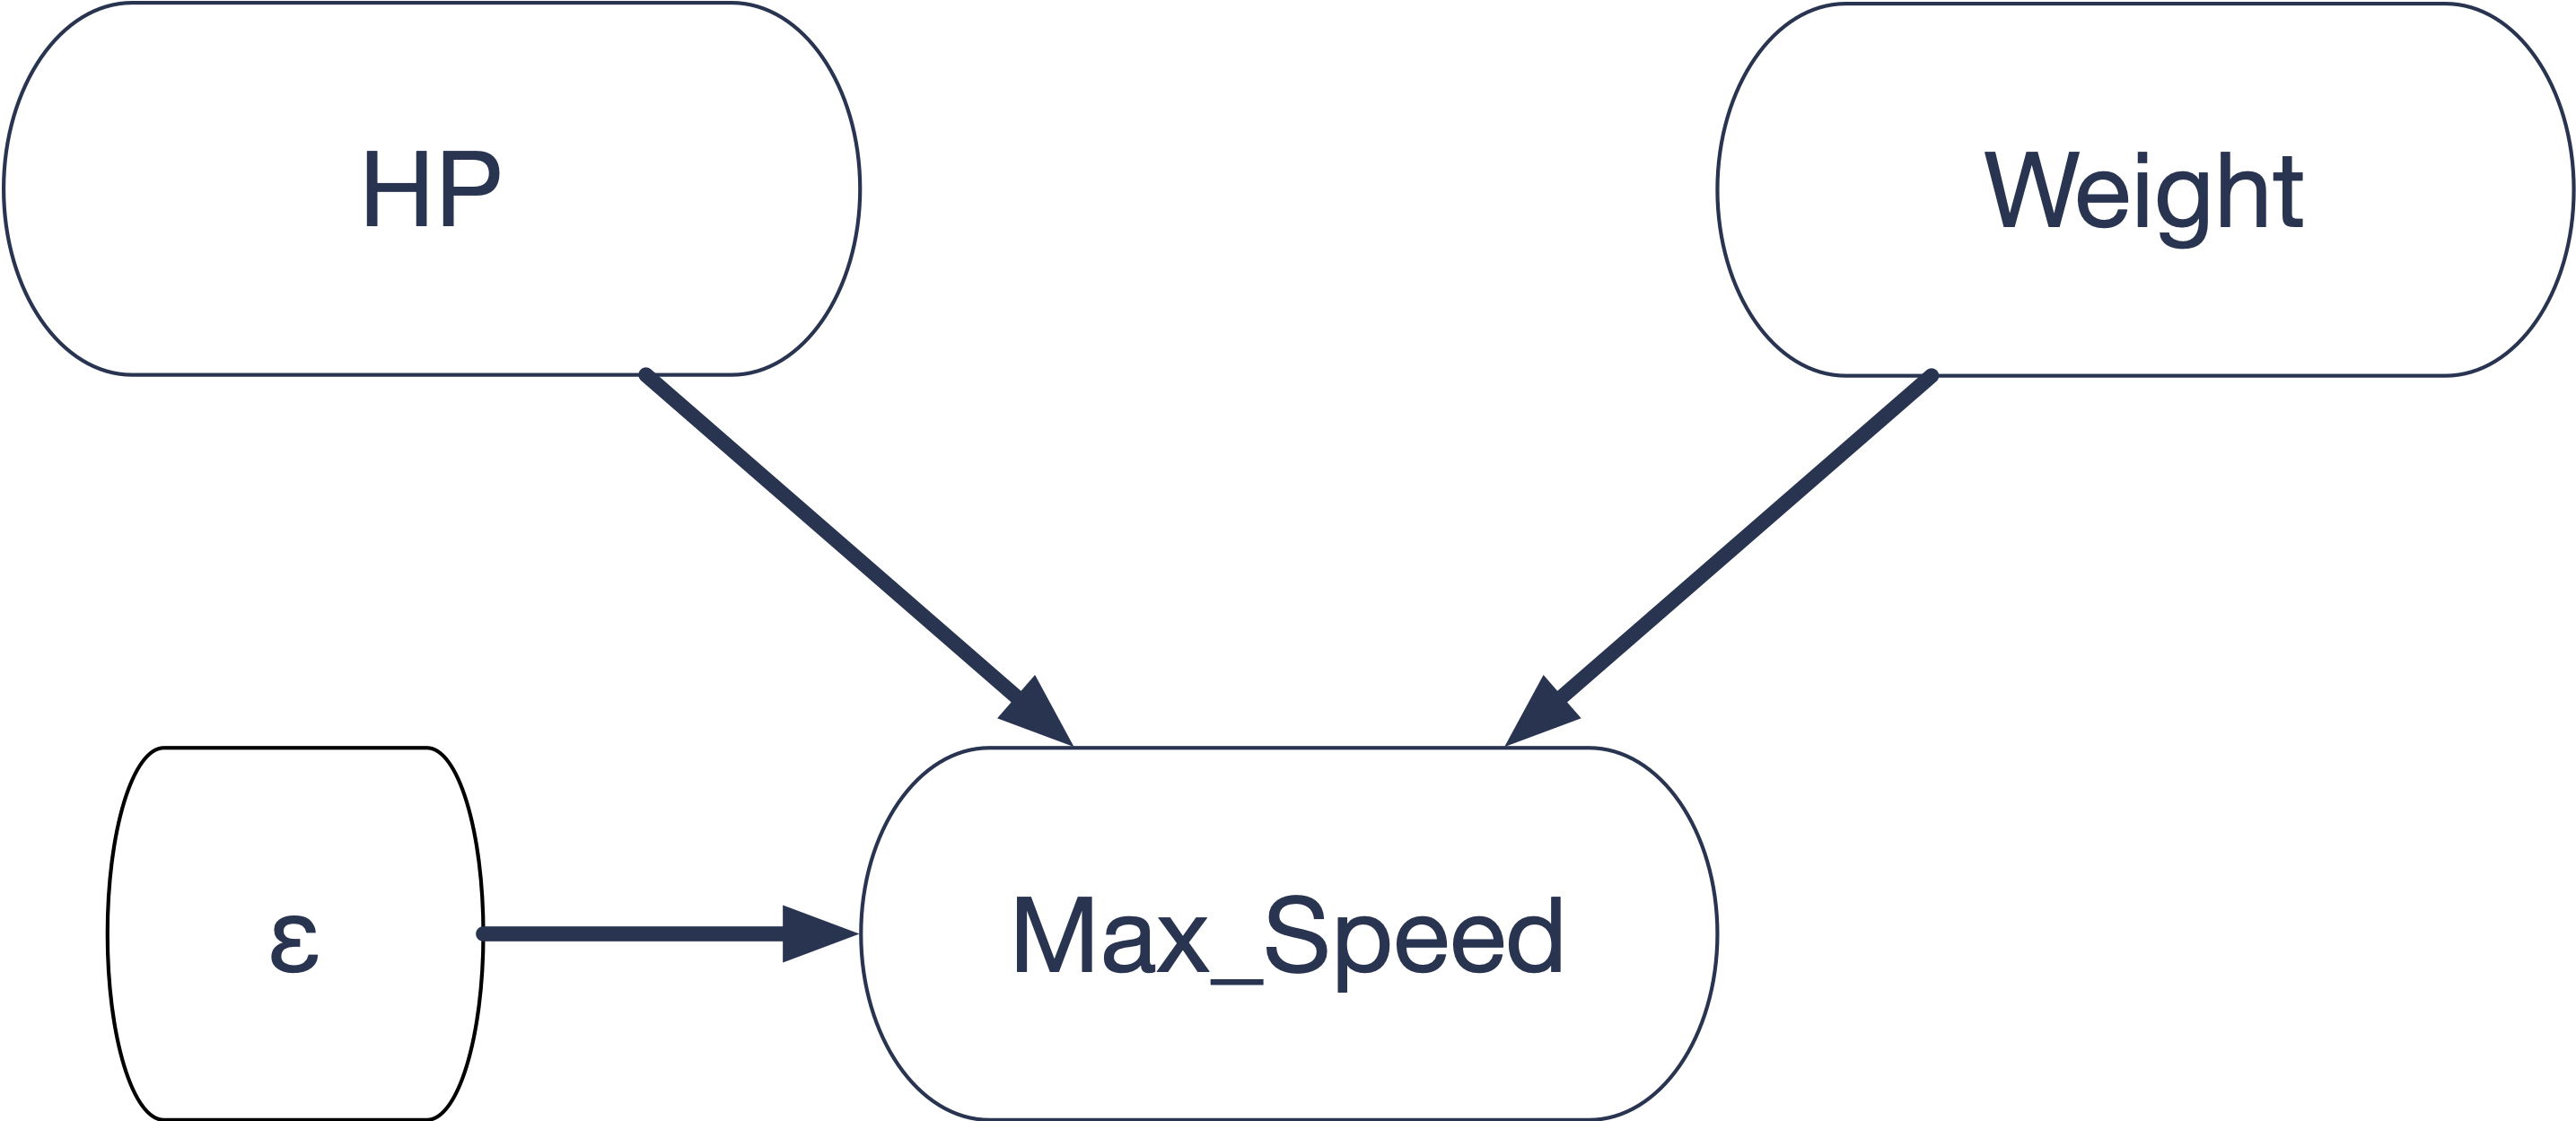
\includegraphics[width = .5\textwidth]{images/causal_graph_base}
\end{center}

\note[]{
  $\epsilon$ and $HP$ have no common ancestors.  $\epsilon$ and
  $Weight$ have no common ancestors.  \\ 
  $\implies \epsilon$ and $HP$ are independent.  So are $\epsilon$ and
  $Weight$. \\ 
$\implies cov(HP,\epsilon) = cov(Weight, \epsilon) =0$ \\ 
$\implies \widehat{Max\_Speed} = \beta_0 + \beta_1 HP + \beta_2
Weight$ is the BLP  \\ 
$\implies$ OLS is consistent for the structural coefficients}
\end{frame}

\section{Applications for the One-Equation Model}

\begin{frame}[standout]
  \frametitle{An Important Question}
  When is the one-equation structural model valid?
  
  \note[item]{We've seen how useful the one-equation structural
    model is. \textbf{if it holds}, \textit{our theory about the
      world is true}, \textbf{then if we use OLS to estimate
      parameters, these parameters will have a causal
      interpretation.}}
  \note[item]{The elephant in the room is that our theory has to
    be true -- a supposition that we will \textit{never} have data
    to directly evaluate.  How do you know when the model is
    credible?}
  \note[item]{There was a time, when researchers believed in the
    one-equation model a lot - or at least they behaved like they did.
    Running OLS regressions, made small tweaks and supposed their
    results held a causal interpretation.} 
  \note[item]{But, this is a bit like Emperor Nero fiddling while Rome
    burns or putting a finger in a dike.} 
  \note[item]{Over time, and with better methods, we've been
    discovering that those old regressions were often far off the
    mark.} 
\end{frame}
  
  
  \begin{frame}[b]
  \frametitle{Confounding Variables in Observational Data}
  \note[item]{Let's talk through one example.  A lot of labor
    economists are interested in this relationship.  From education to
    wage.  Suppose you decide to get an extra year of education, will
    that cause your wage to go up, and by how much?} 
  
  \begin{center}
    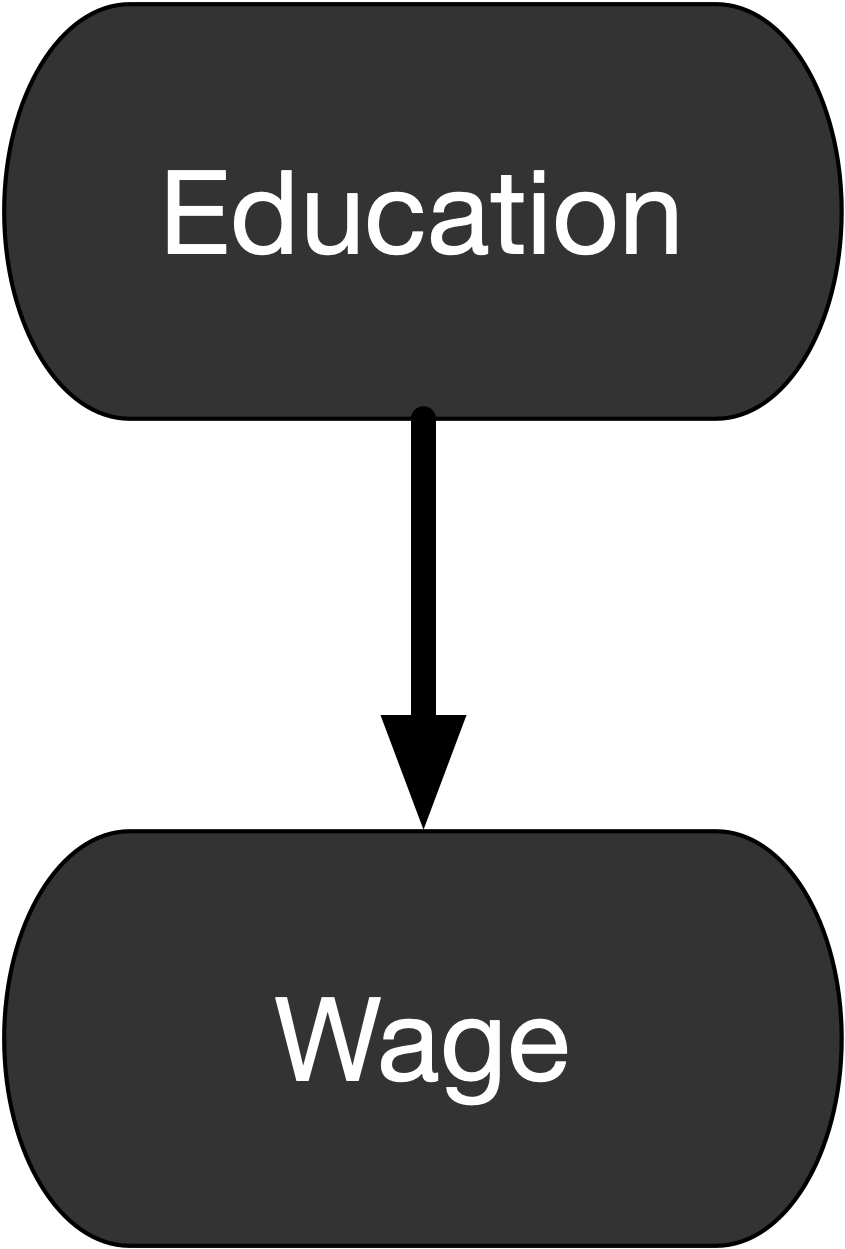
\includegraphics[width=.25\linewidth]{images/education_wage}
  \end{center}
  
  \note[item]{Is this a valid causal graph?  For it to be valid,
    education and wage can't have any common causes.  If they have
    common causes, we'd need to include them in the graph.\paul{draw a
      question mark with two arrows} } 
 
  \note[item]{You can see that the list gets big really quickly:
    \textbf{motivation, parents, financial wealth, positive mentors,
      discrimination based on race, sex, gender, positive teacher
      praise}} 
  \note[item]{Now it's true, if we could measure all these factors and
    put them into the regression, we could the problem. } 
  \note[item]{The problem is that we can't possibly measure all of the
    possible factors.  I'm not sure we could even think of them all.
    And some of these may be impossible to measure.} 
  \note[item]{Nowadays, if you try to measure this effect with an ols
    regression, it's just not credible.  you could never publish work
    like that.} 
  \note[item]{This is really the common case with observational data.
    your default assumption should be that the one-equation model does
    not hold}  
\end{frame}

\begin{frame}
  \frametitle{When Is the One-Equation Model Credible?}
  \note[item]{So when CAN you believe the one-sample model?}
  \note[item]{A few situations make it easy.}
  \begin{itemize}
  \item True experiments
  \item Some natural experiments
  \item Differenced panels
  \end{itemize}
\end{frame}

\begin{frame}
  \frametitle{The True Experiment}
  
  \note[item]{A true experiment is considered the gold standard for
    measuring causal effects.} 
  \note[item]{One way to think about it, is you're using randomness to
    break links in the causal graph } 
  \note[item]{In a true experiment, you can divide variables into
    three classes.} 

  \begin{columns}
    \begin{column}{0.6\textwidth}
      \begin{itemize} 
      \item Treatment $T$ is randomly assigned (e.g. coin flip)
        $\implies$  no incoming paths \textit{other than the coin}.
      \item Controls $C_1, C_2, C_3$ are either measured or determined before
        treatment
        \begin{itemize}
        \item No paths from $T$ to controls, or controls to $T$
        \end{itemize}
      \item Outcome $Y$ measured after $T$
      \end{itemize} 
    \end{column}
    
    \begin{column}{0.4\textwidth} 
      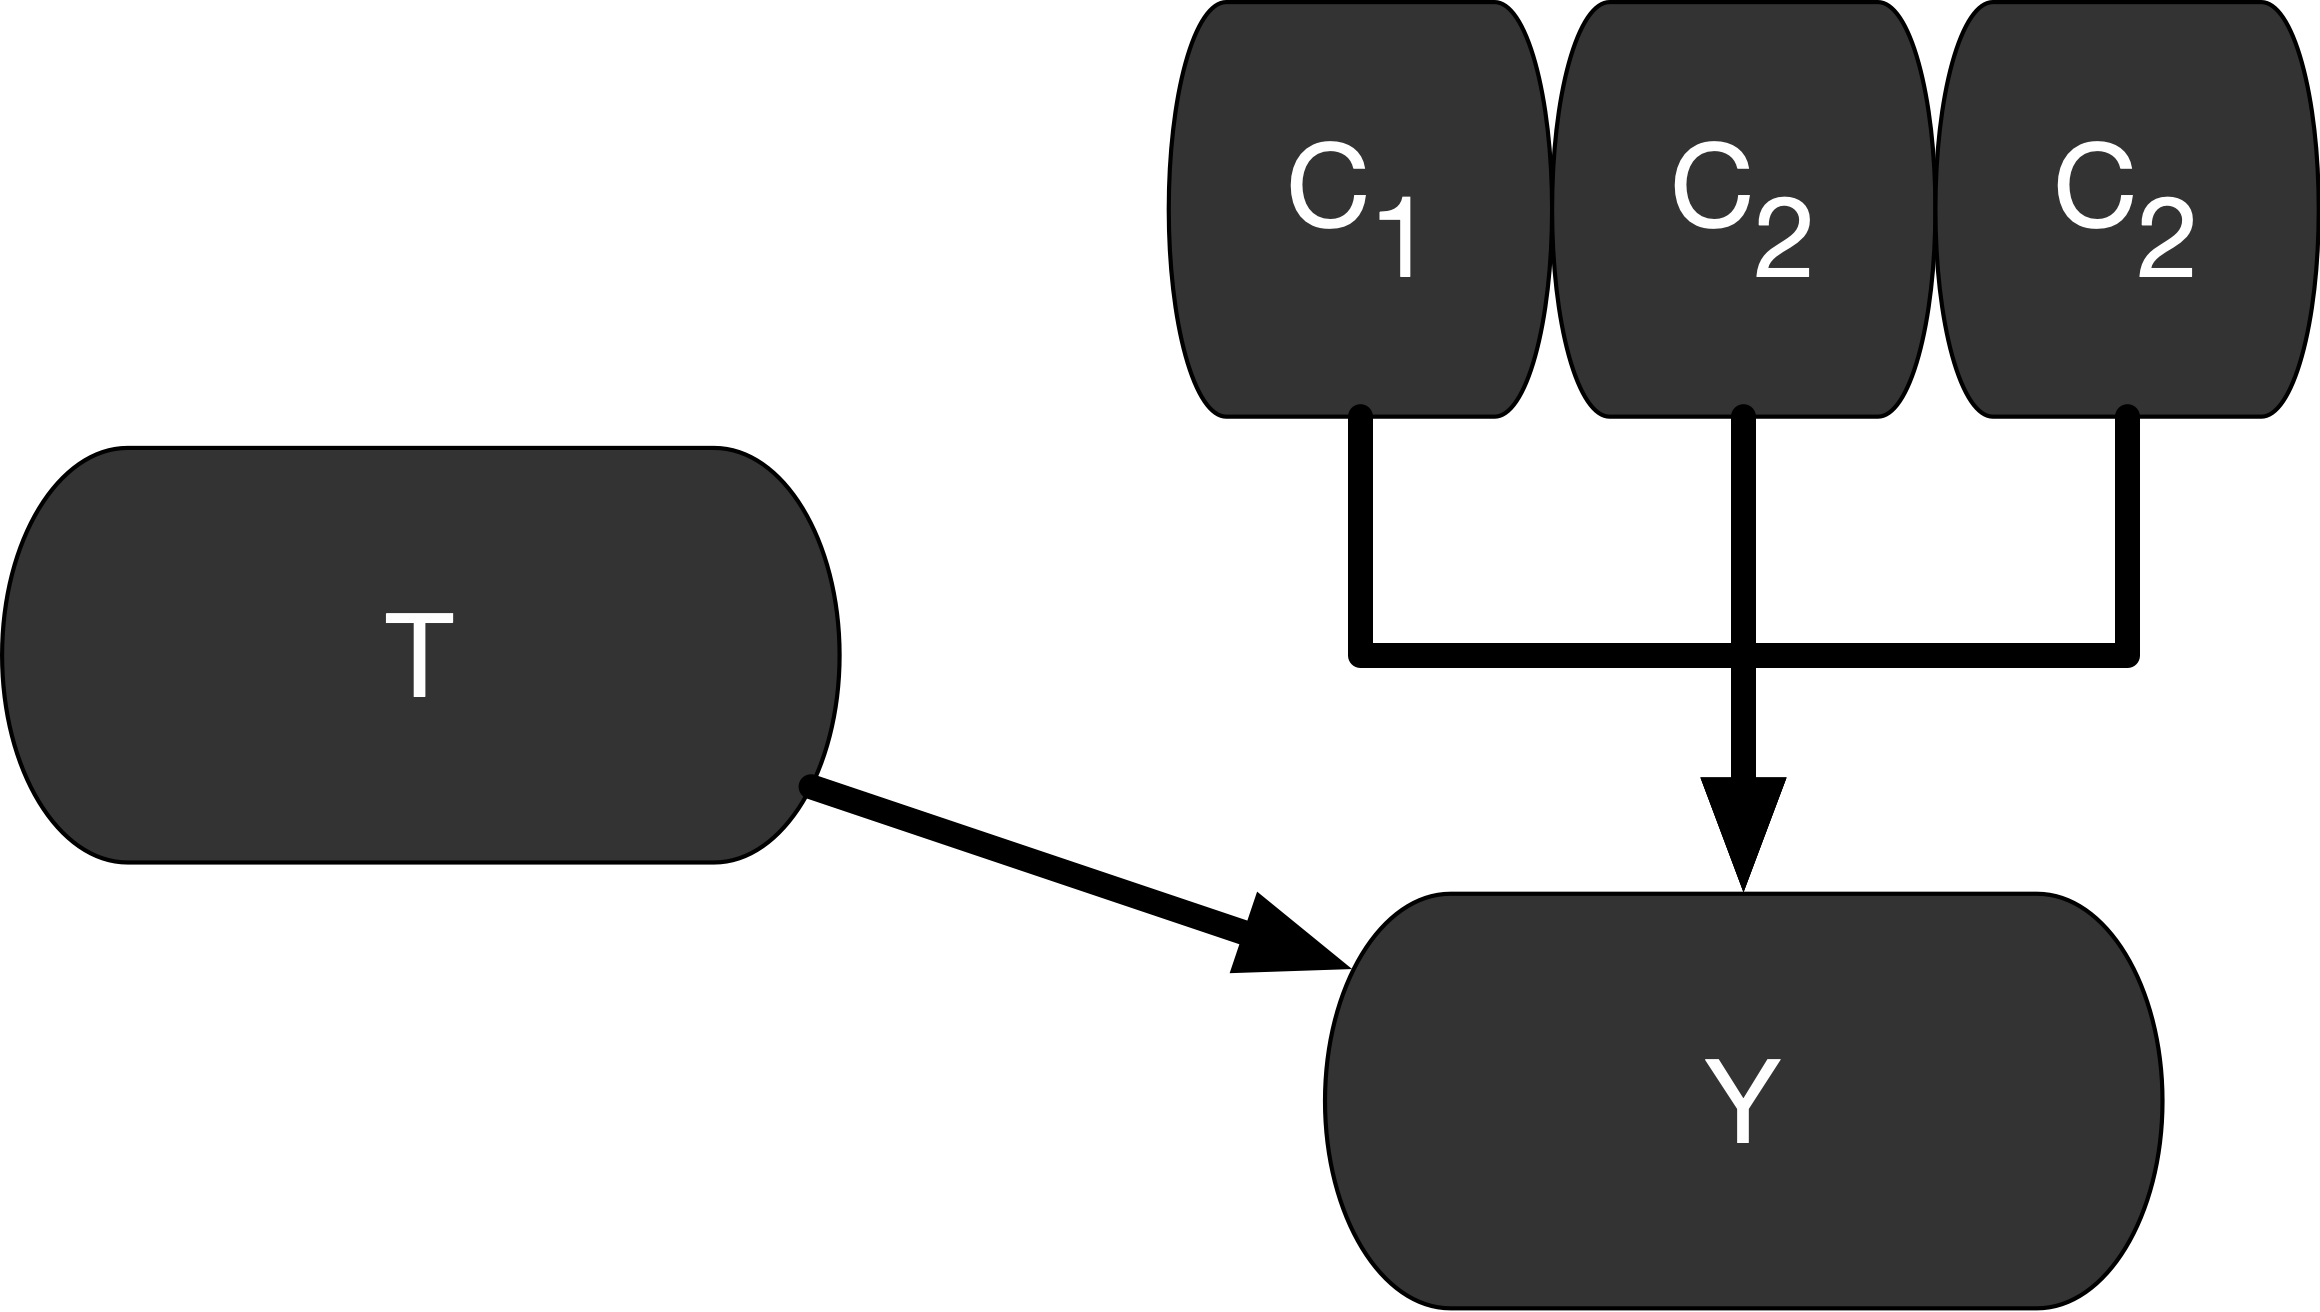
\includegraphics[width = \textwidth]{images/experiment.png}
      
    \end{column}
  \end{columns}
  
  \vspace{.5cm}
  $\implies$ OLS consistent estimates effect of $T$ on $Y$.
\end{frame}

\begin{frame}
  \frametitle{Some Natural Experiments}
  
  \textbf{Natural experiment:} A scenario in which we can exploit
  naturally occurring variation to estimate structural parameters 
  
  \begin{itemize}
  \item Often through instrumental variables, regression discontinuity,
    or other advanced techniques  
  \item May enable OLS to \textit{identify} causal quantities if
    treatment is random
    
    \begin{itemize}
    \item The Vietnam War lottery
    \item Tropical cyclones
    \item Forest fires
    \item Network outages
    \end{itemize}
  \end{itemize}
  
  \note[item]{There could be general trends, but if we stick to one
    cross section, and compare areas hit by a cyclone against areas
    that aren't hit, we may argue that there can't be many confounding
    variables.} 
\end{frame}

\begin{frame}
  \frametitle{Differenced Panels}
  
  \centering
      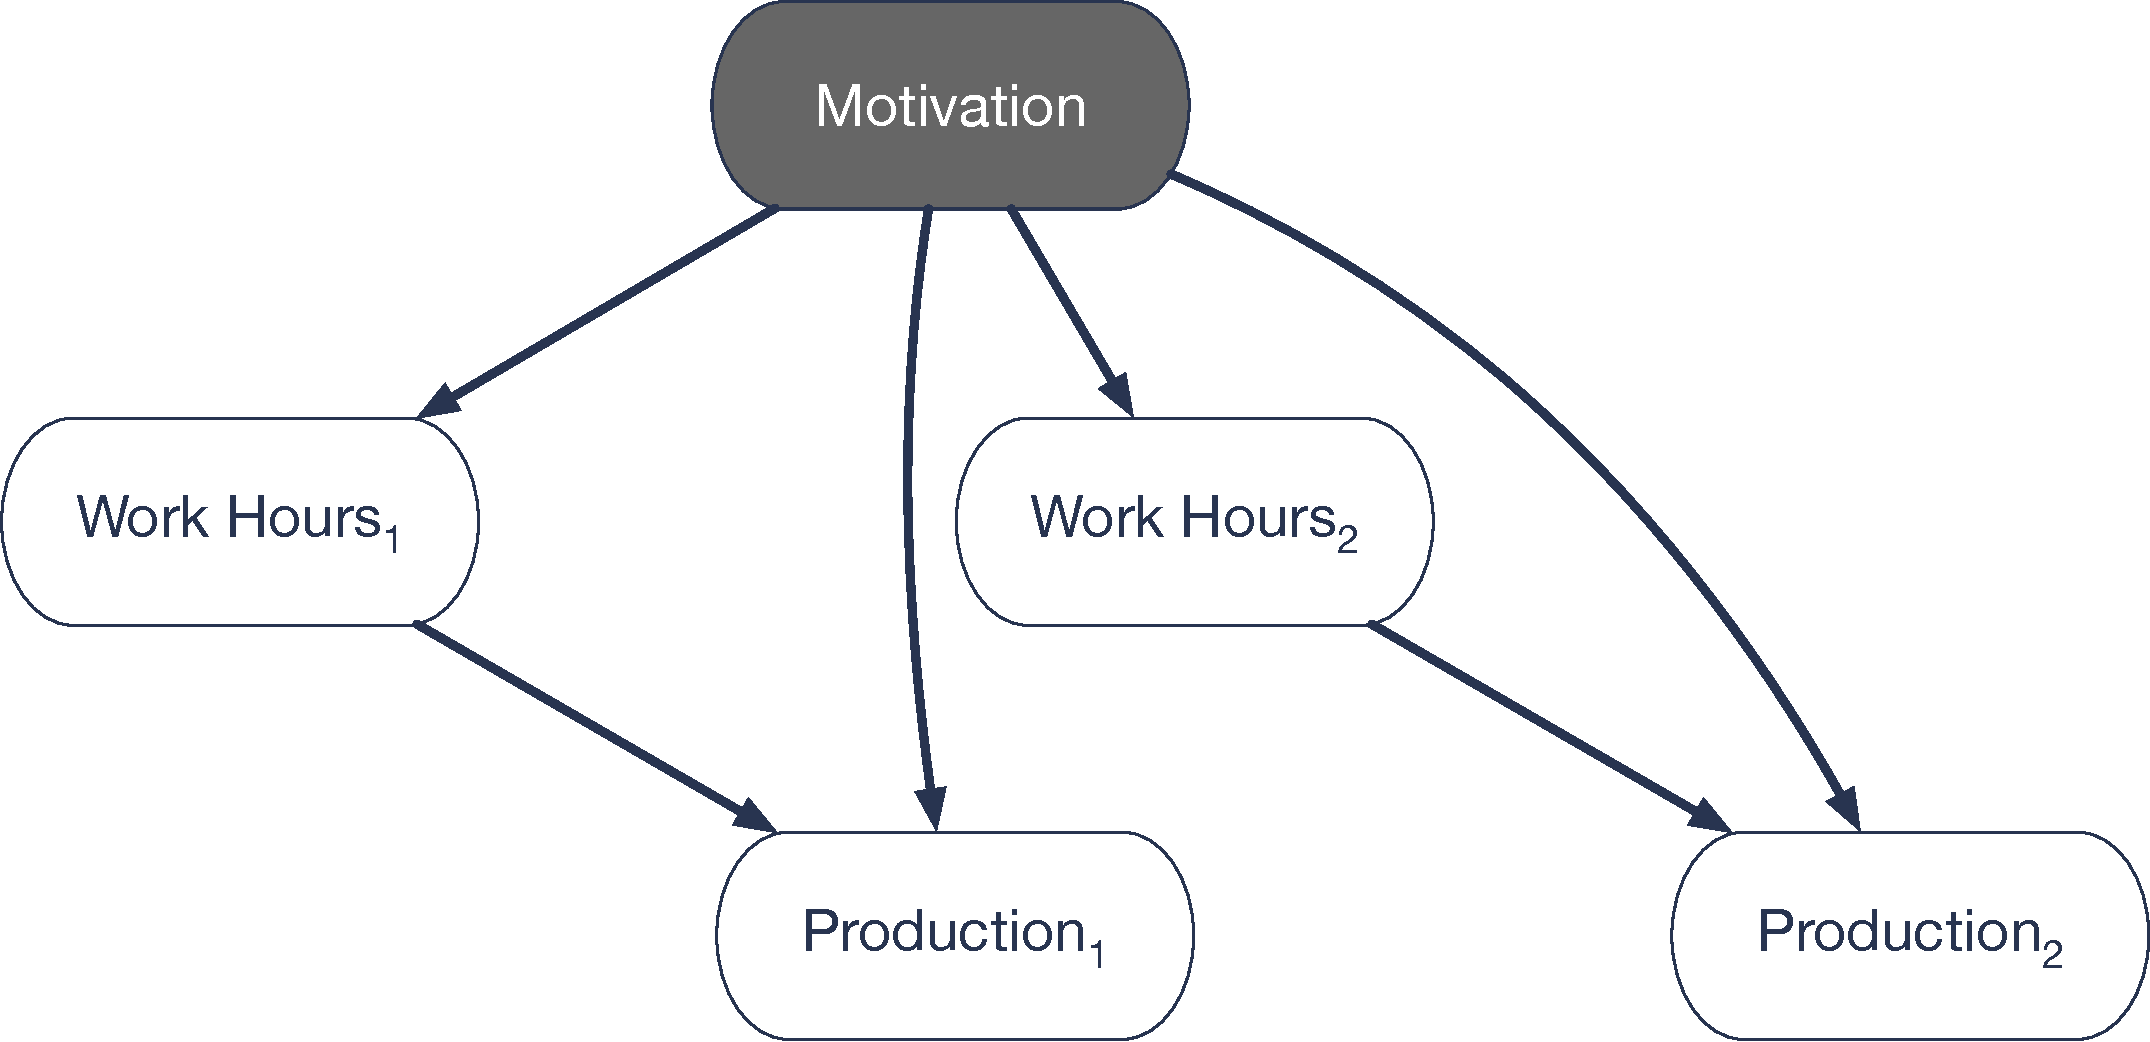
\includegraphics[width = .5\linewidth]{images/motivation_productivity}
  
  \note[item]{This is what we call a diff-in-diff design.  our outcome
    is differences in productivity, and we're looking at the differences
    in that variable across people.  diff-in-diff.}  
  
  \begin{align*}
    Production_1 &= \beta_0 + \beta_1 Work\_Hours_1 + \beta_2 Motivation + \epsilon_1\\
    -\Bigg[ Production_2 &= \beta_0 + \beta_1 Work\_Hours_2 + \beta_2 Motivation + \epsilon_2 \Bigg]\\
    \hline
    \Delta Production &=  \qquad \beta_1 \Delta Work\_Hours \qquad
                          \qquad + (\epsilon_{1} - \epsilon_{2})
  \end{align*}
  \note[item]{Confounding variables may be constant over time}
  \note[item]{Suppose that we have data for $t \in {1,2}$.}
  \note[item]{Note:  Cannot eliminate non-constant confounders}
  \note[item]{But: what if Motivation in period 2 changes, depending on
    the work hours in period 1?} 
  \note[item]{So cannot help if the confounders change} 
  \note[item]{and it cannot help if there is reverse causality.} 
  \note[item]{But still, this design can be reasonably convincing in
    some scenarios.} 
 
\end{frame}


\section{Violations of the One-Equation Structural Model} 

\section{Omitted Variables}

\begin{frame}
  \frametitle{Omitted Variables}
  
  \begin{columns}[t]
    \column{0.5\textwidth}
    \begin{block}{Assumed Model}
      Education causes wages
    \end{block}
    \centering
    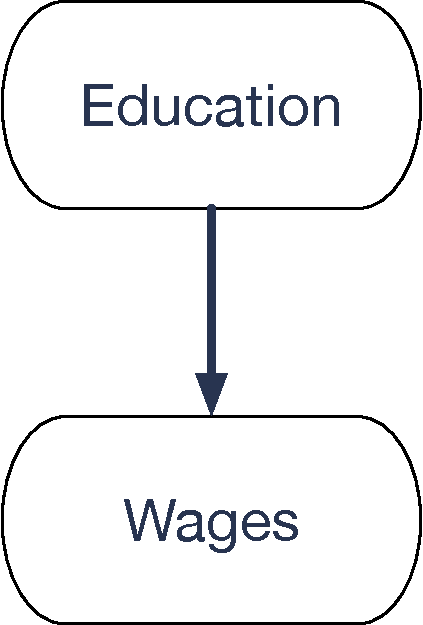
\includegraphics[width=3cm]{images/education_assumed}
    
    \column{0.5\textwidth} 
    \begin{block}{True Model} 
      Motivation causes both education and wages
    \end{block}
    \centering
    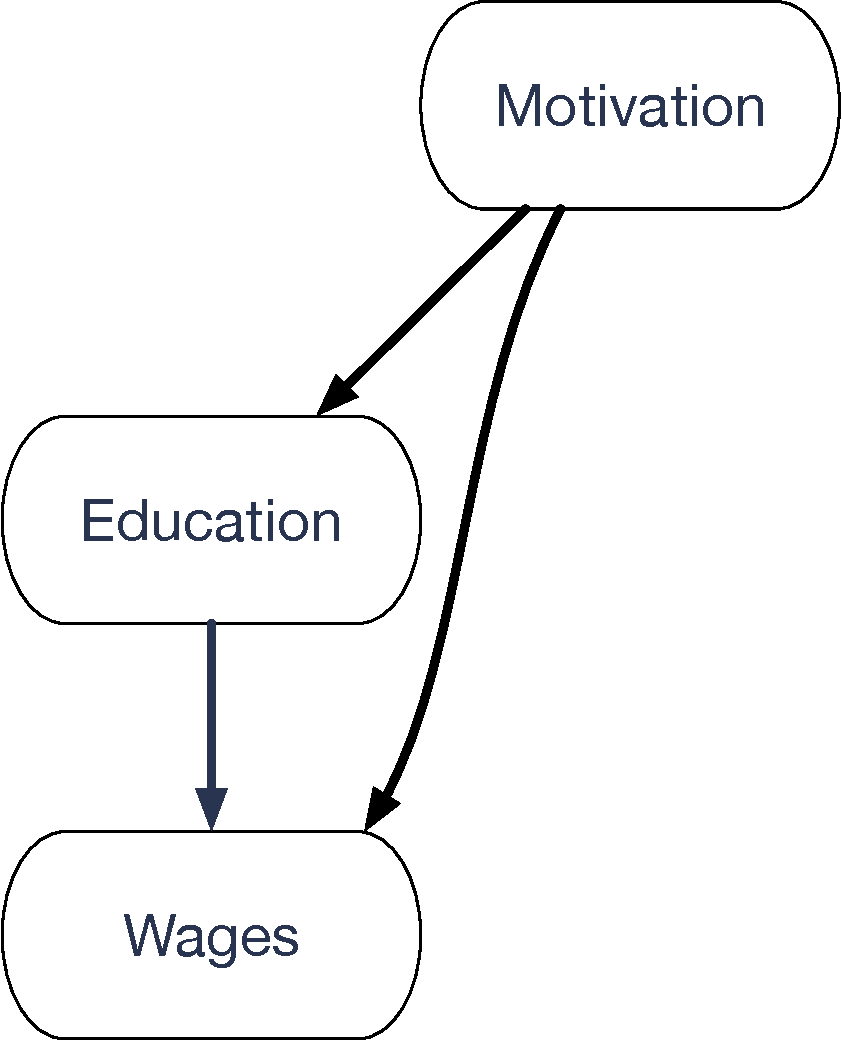
\includegraphics[width=3cm]{images/education_true}
  \end{columns}
  
  \note[item]{When you do explanatory modeling, you work inside a causal theory.  You want your theory to be right, but you always worry that it may not be exactly right.  In particular, there could be causal pathways that you should have included, that you didn't include.}
  \note[item]{That means that there's an extra step in your analysis.  you need to consider what the most likely errors in your causal graph might be.  and reason about how they might bias your estimates.}
  \note[item]{In the case of the one-sample model, there are a couple of common violations that you need to watch out for.  The violation is what we call an omitted variable.}
  \note[item]{It turns out that when we have an omitted variable, ols regression will not estimate the correct target!}
\end{frame}

\begin{frame}
  \frametitle{Omitted Variables}
  % 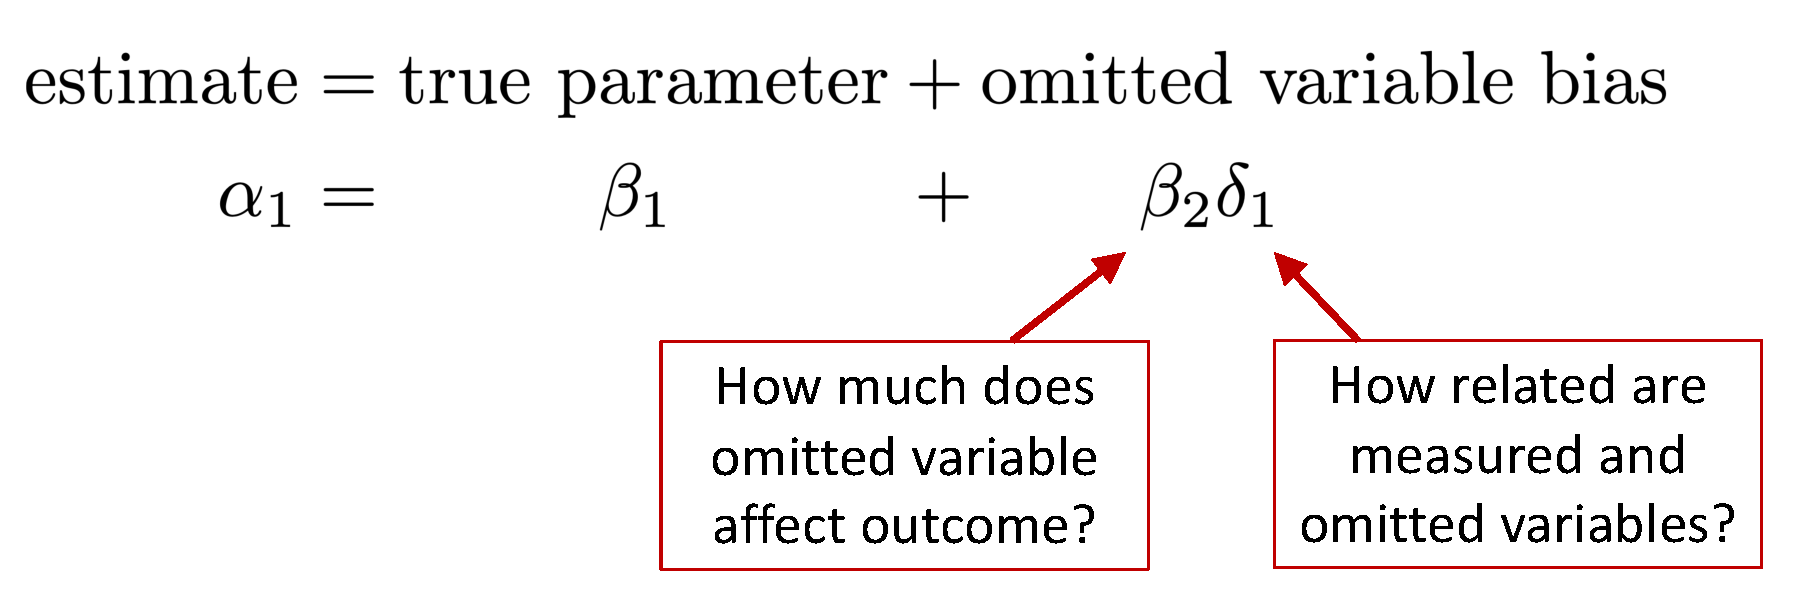
\includegraphics[width = \textwidth]{images/ovb}

    \begin{columns}[t]
     \column{0.45\textwidth}
    \begin{block}{We fit}
   \vspace{.1cm}        $ W  = \tilde{\beta}_0 + \tilde{\beta}_1  E + \tilde \epsilon$
    \end{block}
    \column{0.55\textwidth}
    \begin{block}{True structural equation}
  \vspace{.2cm}     $W = \beta_0 + \beta_1 E + \beta_2 M + \epsilon$
    \end{block}
    \end{columns}
    \vspace{1cm}
    
  \begin{itemize}
  \item We are interested in $\beta_1$.
  \item What is the bias, $E[\tilde \beta_1 - \beta_1]$?
  \end{itemize} 
  \note[item]{We want to know this bias.  I'll show you how to calculate it.}
\end{frame}

\begin{frame}[t]
  \frametitle{Omitted Variable Bias in Simple Regression}
    \begin{columns}[t]
     \column{0.45\textwidth}
    \begin{block}{We fit}
   \vspace{.1cm}        $ W  = \tilde{\beta}_0 + \tilde{\beta}_1  E + \tilde \epsilon$
    \end{block}
    \column{0.55\textwidth}
    \begin{block}{True structural equation}
  \vspace{.2cm}     $W = \beta_0 + \beta_1 E + \beta_2 M + \epsilon$
    \end{block}
    \end{columns}
%    
%  \begin{align*}
%    W &= \beta_{0} + \beta_{1} E + \beta_{2} M + \epsilon \tag{True} \\ 
%    W &= \tilde{\beta}_{0} + \tilde{\beta}_{1} E + \epsilon \tag{Estimated} 
%  \end{align*}

Regress $M$ on $E$:
$$M = \delta_0 + \delta_1 E + \nu$$

Consider two quantities
\begin{itemize}
\item $\beta_2$ is the effect of $M$ on $W$.
\item $\delta_1$ represents how related $M$ and $E$ are.
\end{itemize}

 \textbf{Omitted Variable Bias:} $ \tilde{\beta}_{1}  - \beta_{1} = \beta_{2} \delta_{1} $
\end{frame}




 
 \begin{frame}
  \frametitle{Omitted Variable Bias in Multiple Regression}
    \begin{columns}[t]
     \column{0.45\textwidth}
    \begin{block}{We fit}
   \vspace{.1cm}      $  Y = \tilde{\beta}_0 + \tilde{\beta}_1 X_1 + \tilde{\beta}_2 X_2  + ...  $
   
   $\qquad + \tilde{\beta}_{k-1} X_{k-1}   + \tilde \epsilon$
    \end{block}
    \column{0.55\textwidth}
    \begin{block}{True structural equation}
  \vspace{.2cm}     $Y  = \beta_0 + \beta_1 X_1 + \beta_2 X_2 + ... $
  
  $\qquad +\tilde{\beta}_{k-1} X_{k-1} +  \beta_k X_k + \epsilon  $
    \end{block}
    \end{columns}
    
    


  \note[item]{The fit model omits $X_{k}$}
  
Regress $X_k$ on other $X$'s:
$$  X_k = \delta_0 + \delta_1 X_1 + ... + \delta_{k-1} X_{k-1} + \nu$$

    \textbf{Omitted Variable Bias:}  $\tilde{\beta}_{1} -  \beta_1 =  \beta_{k}\delta_1$


    \note[item]{As you can see, the formula for OVB is the same.  Once
      again, you should think about $\delta_1$ as the strength of the
      relationship between the measured and omitted vars.} 
    \note[item]{But I should qualify that a little bit.  $\delta_1$ is in
      a multiple regression..   And some surprising things can happen in a
      multiple regression. For example the measured and omitted could have
      a positive correlation, but when you add the other variables to the
      regression, the sign could flip.  Even though that's possible, it's
      really hard to predict.  So really, I want you to remember the rule
      of thumb: $\delta_1$ represents the strength of the relationship
      between the measured and omitted vars. } 
  \end{frame}



\begin{frame}
  \frametitle{Estimating Omitted Variable Bias}
  
     \begin{center}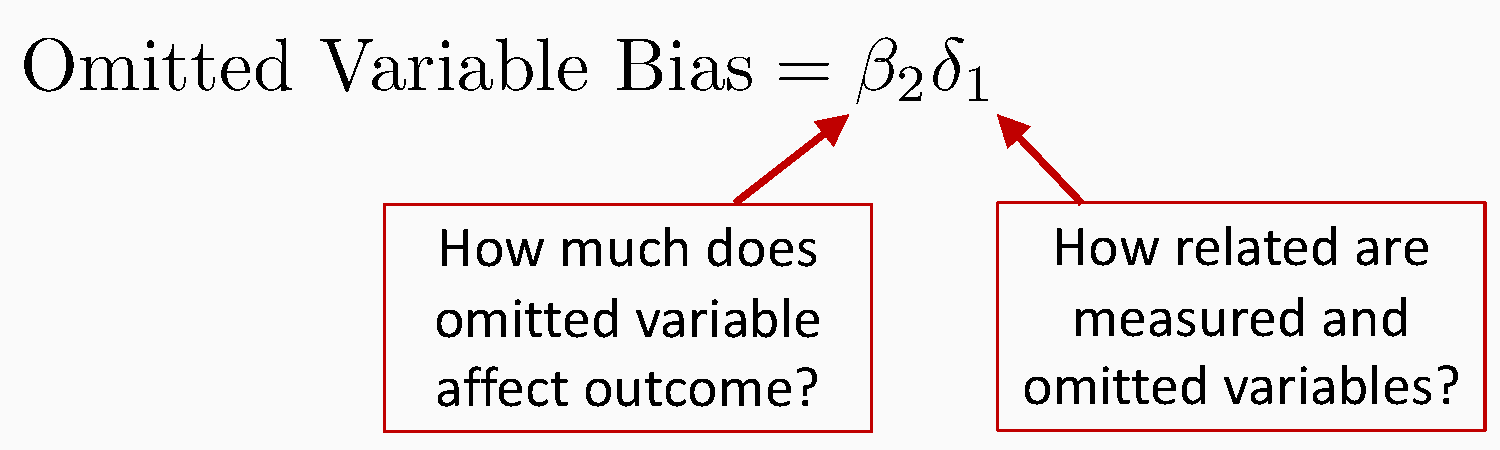
\includegraphics[width = .8\textwidth]{images/ovb_2}
  \end{center}
  
  \note[item]{By definition, we never know what our omitted variable
    bias is - the omitted variable is omitted.} 
  \note[item]{But actually, you can sometimes use your background
    knowledge to estimate the bias} 
  \note[item]{Not very accurately.  But at the least, you can estimate
    whether the bias is positive or negative, and that's actually
    pretty helpful.  You especially want to know if its pushing your
    coefficient towards zero or away from zero.} 
  
\vspace{1cm}
We fit:  $\widehat{Wage} = \tilde{\beta}_0 + \tilde{\beta}_1 Education$; \hspace{.1cm}Omitted: $Motivation$

\note[item]{In the wage equation, we mivght estimate the $M$ and $W$
  have a + relationship.  $M$ and $E$ have a + relationship.  so $OMB
  = ++ = +$ } 
\note[item]{The coefficient $\alpha_1$ is also +, so the bias is
  pushing it away from zero.} 

\note[item]{Take a moment and think about this.  which is worse, bias
  towards zero or away from zero.} 

\note[item]{The answer is, it's usually worse to have bias away from
  zero.  That's because the true effect is closer to zero, so we don't
  know how much of the relationship we see is real and how much is
  bias.  it might even be that the real effect is zero, or in the
  other direction. } 
\end{frame}

\begin{frame}[t]
  \frametitle{Assessing Omitted Variable Bias}
 \vspace{2cm} Which is worse: Bias toward zero or bias away from zero?
\end{frame}

\section{Proof of Omitted Variable Bias}


\begin{frame}[t]
  \frametitle{The Omitted Variable Bias in Simple Regression}
    \begin{columns}[t]
     \column{0.45\textwidth}
    \begin{block}{We fit}
   \vspace{.1cm}        $ W  = \tilde{\beta}_0 + \tilde{\beta}_1  E + \tilde \epsilon$
    \end{block}
    \column{0.55\textwidth}
    \begin{block}{True structural equation}
  \vspace{.2cm}     $W = \beta_0 + \beta_1 E + \beta_2 M + \epsilon$
    \end{block}
    \end{columns}


    \note[item]{Draw each of the following} 
    \note[item]{$E[\epsilon] = 0$} 
    \note[item]{$cov[E,\epsilon] = 0$}
    \note[item]{ $cov(M,\epsilon) = 0$}
    
    
  \note[item]{$\tilde{\beta}_1 = \frac{cov[W,E]}{var[E]} =  \frac{cov[\beta_0 + \beta_1 E + \beta_2 M + \epsilon,E]}{var[E]} $}
  \note[item]{$  \frac{\beta_1 var[E]  + \beta_2 cov[M,E]}{var[E]}  = \beta_1 +  \frac{ \beta_2 cov[M,E]}{var[E]} $}
  \note[item]{What is the second term?  it looks like the formula for a regression coefficient.  But what regression?}
  \note[item]{$M = \delta_0 + \delta_1 E + v$}
  \note[item]{$\tilde \beta_1 = \beta_1 + \beta_2 \delta_1$}
 \end{frame}

% \section{Learnosity Check}

% \begin{frame}
%   \frametitle{Estimating Omitted Variable Bias}

%   In the following equation, estimate whether the omitted variable
%   bias is towards zero or away from zero.
%   $ \widehat{Air\_Purity} =  .97 - .00034 \ Bicycles\_per\_Square\_Mile$
%   Omitted: People per Square Mile
%  \note[item]{\alex{We should totally have them code this as well.}}
% \end{frame}

\section{Reverse Causality}

\begin{frame}[t]
  \frametitle{Reverse Causality}
  % \begin{block}{Variables} 
  %   Education ($E$), Wage ($W$)
  % \end{block} 
  
  \begin{columns}[t]
    \column{0.5\textwidth}
    \begin{block}{Assumed model}
      Education causes wages
    \end{block}
    \vspace{2em}
    \centering
    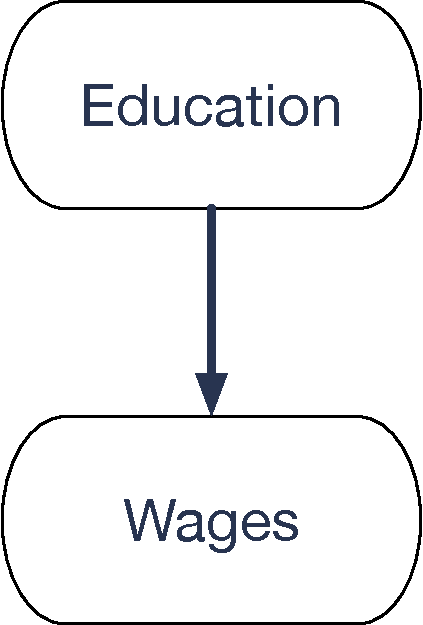
\includegraphics[width=0.6\textwidth]{images/education_assumed}
    \column{0.5\textwidth}
    \begin{block}{True model}
      Education causes wages \textit{and} wages cause education
    \end{block}
    \centering
    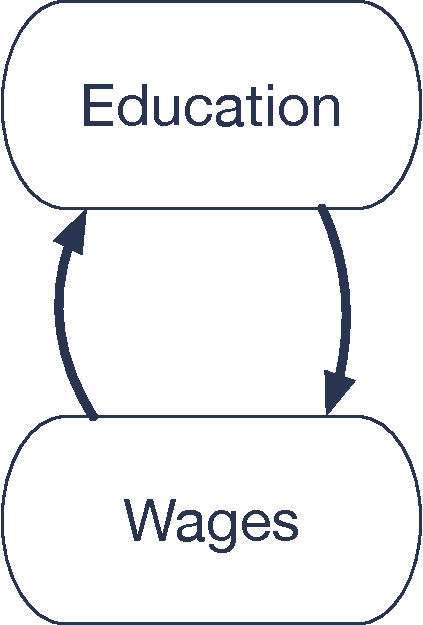
\includegraphics[width=0.6\textwidth]{images/reverse_causality}
  \end{columns}
  
  \note[item]{What if having a higher wage allows people to pay for
    more education.}  
  \note[item]{Feedback}
  
\end{frame}



\begin{frame}
  \frametitle{An SEM Version}
  
  \begin{columns}
    \begin{column}{0.5\textwidth}
      \center
      True structural equations:
      \begin{align}
        W &= \beta_0 + \beta_1 E + \epsilon_1\\
        E &= \gamma_0 + \gamma_1 W + \epsilon_2
      \end{align}
    \end{column}
    \begin{column}{0.5\textwidth} 
      \center
      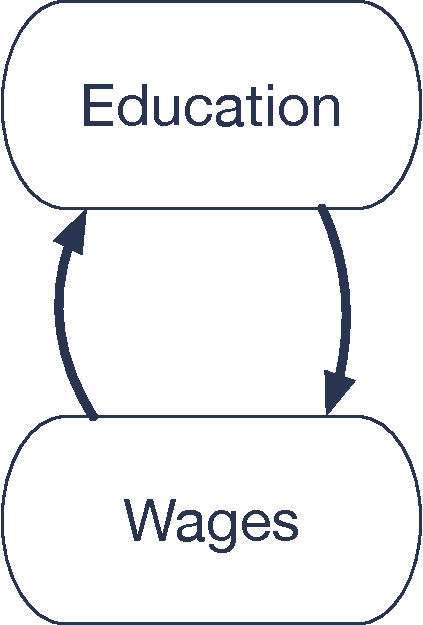
\includegraphics[height = 3cm]{images/reverse_causality}
    \end{column}
  \end{columns}
  
  \note[item]{If we additionally assume that all the responses are linear, we get an SEM that looks like this.}
  \note[item]{In our previous model, the structural equation always coincided with the BLP.  But that's not true here. }
  \note[item]{That's because $E$ and $\epsilon_1$ are not independent.  If I draw $\epsilon_1$ here, you can see that $E$ is a descendant, so they'll be correlated.}
  \note[item]{So what is the BLP?  We have to solve this system of equations...}
  
  Observations
  \begin{itemize}
  \item E is a descendant of $\epsilon_1$.
  \item $\implies$ $E$ and $\epsilon_1$ are dependent.
  \item $\implies$ (1) is not the BLP.
  \end{itemize}
  
  Since OLS estimates the BLP, it can't estimate (1).
\end{frame}

\begin{frame}
  \frametitle{Understanding Feedback}
    \begin{columns}
    \begin{column}{0.5\textwidth}
      \center
      True structural equations:
      \begin{align*}
        W &= \beta_0 + \beta_1 E + \epsilon_1\\
        E &= \gamma_0 + \gamma_1 W + \epsilon_2
      \end{align*}
    \end{column}
    \begin{column}{0.5\textwidth} 
      \center
      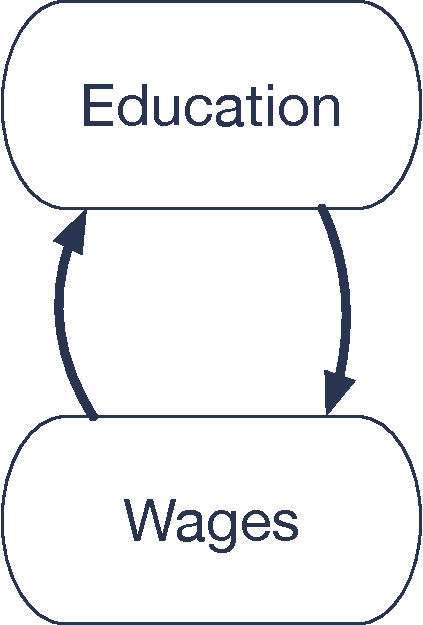
\includegraphics[height = 3cm]{images/reverse_causality}
    \end{column}
  \end{columns}
  Suppose $\beta_1 > 0$
  
  \begin{itemize}
\item Positive feedback $\gamma_1 > 0$ 
\begin{itemize}
\item $\tilde \beta_1 > \beta_1$
\end{itemize}
\item Negative feedback $\gamma_1 < 0$ 
\begin{itemize}
\item $\tilde \beta_1 < \beta_1$
\end{itemize}
\end{itemize}

\end{frame}


\begin{frame}
  \frametitle{Understanding the SEM Equilibrium}

  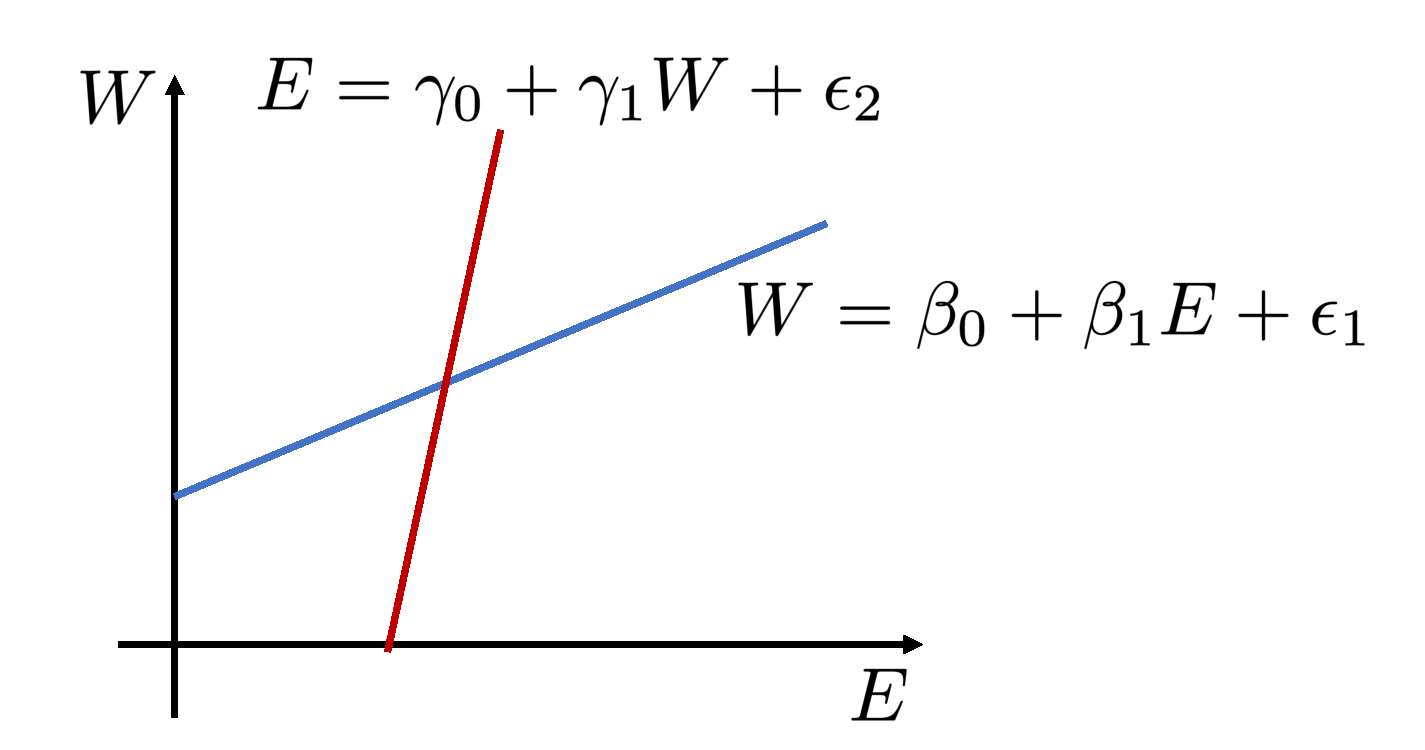
\includegraphics[width =\textwidth]{images/reverse_1}

  \note[item]{As we're talking through this, we need to highlight the
    following:}
  \note[item]{Our theory suspects that these functions are related to
    one another. But, we \textit{really} want to know the causal
    effect of one thing on the other.}
  \note[item]{This means that we have to look for circumstances where
    we have a random shock to the system where we can look at the
    consequences. For example, suppose that we gave out \$5k
    scholarships which made people random sign up for college?} 
\end{frame}

\begin{frame}
  \frametitle{Understanding the SEM Equilibrium}  
   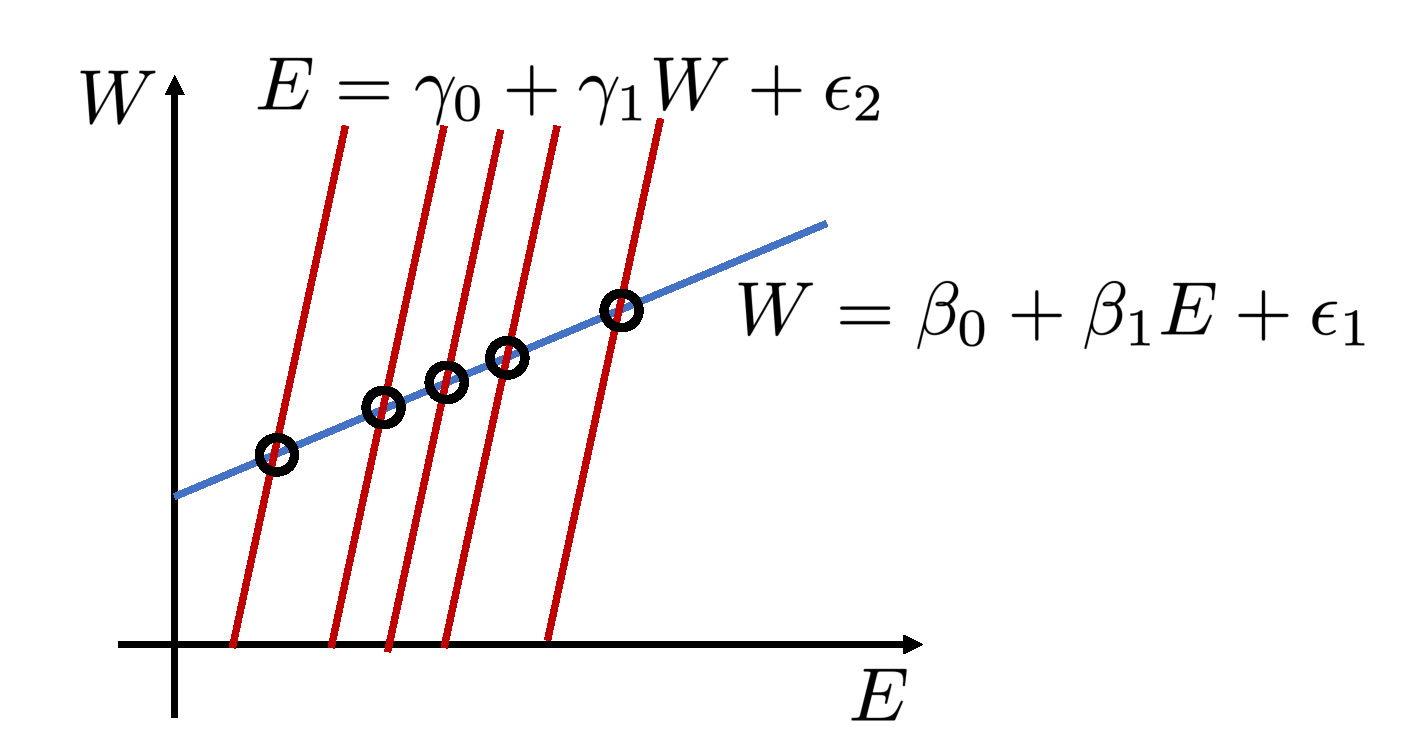
\includegraphics[width =\textwidth]{images/reverse_2}
\end{frame}

\begin{frame}
  \frametitle{Understanding the SEM Equilibrium}
   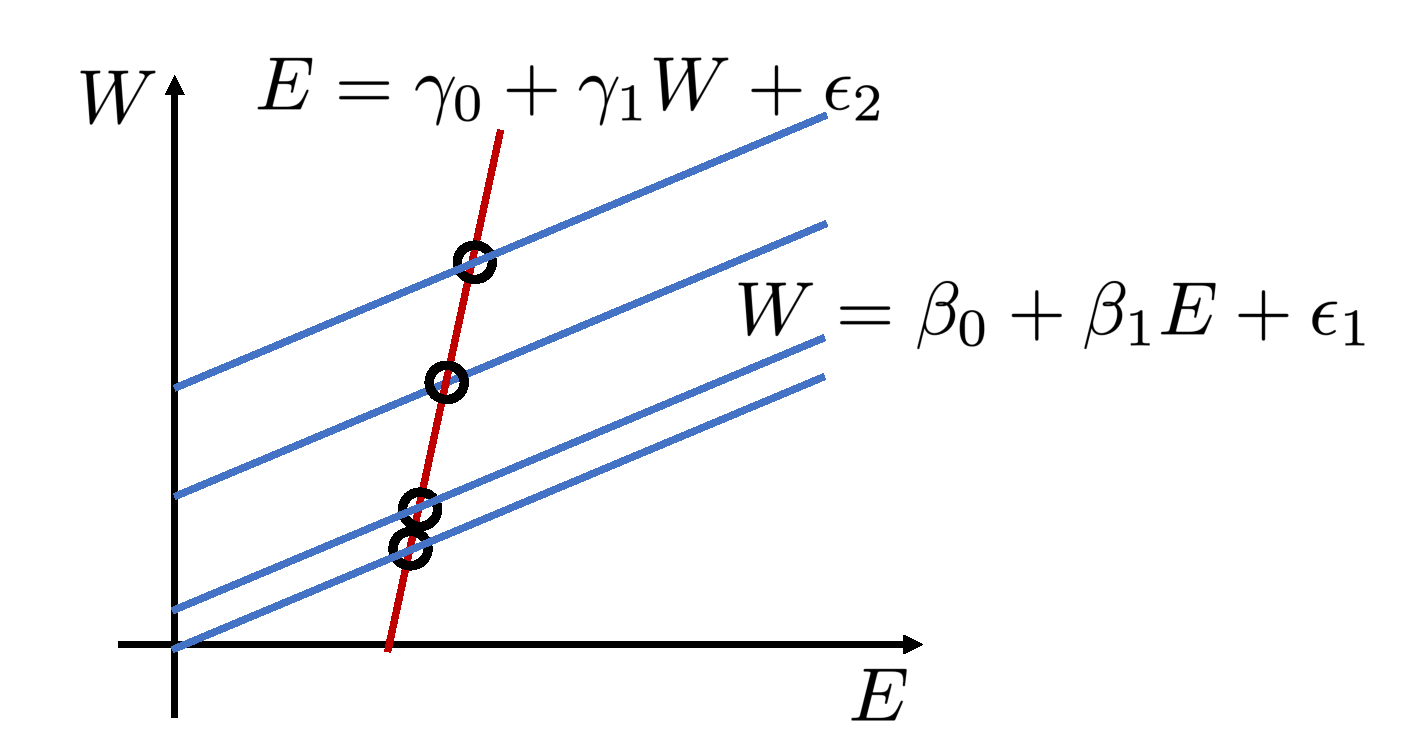
\includegraphics[width =\textwidth]{images/reverse_3}  
\end{frame}


% \begin{frame}
%   \frametitle{Solving for the BLP}
% Solve for W and E:
% \begin{align*}
%     W &= \frac{\beta_0 + \beta_1 \gamma_0 + \beta_1 \epsilon_2 + \epsilon_1}{1-\beta_1\gamma_1}\\
%     E &= \frac{\gamma_0 + \beta_0 \gamma_1  + \gamma_1 \epsilon_1 +  \epsilon_2}{1-\beta_1\gamma_1}
%     \end{align*}
% We fit:  $\hat{W} = \alpha_0 + \alpha_1 E$.

% $$\alpha_0 = \frac{cov[W,E]}{ var[E]} = \frac{\gamma_1 var[\epsilon_1] + \beta_1 var[\epsilon_2]}{\gamma_1^2 var[\epsilon_1] + var[\epsilon_2]}$$

% \begin{itemize}
% \item  If $var[\epsilon_2] >> var[\epsilon_1]$, $\alpha_1$ approaches $\beta_1$ (no bias)
% \item  If $var[\epsilon_2] << var[\epsilon_1]$, $\alpha_1$ approaches $1/\gamma_1$
%  \item In general, $\alpha_1$ is between $\beta_1$ and $1/\gamma_1$

% \end{itemize}
% \end{frame}
  
% \section{Learnosity Check}

% \begin{frame}
%   \frametitle{Direction of Reverse Causality Budget}

%   \textbf{Note: This is a Learnosity Activity. We are just placing it
%     here for organization.}

%   In this causal graph, $P$ is number of police, $C$ is number of
%   crimes. You run a regression of crime on police.  is the direction
%   of bias due to reverse causality positive or negaitve?
% \end{frame}

\section{Outcome Variables on Right-Hand Side}


\begin{frame}
  \frametitle{Outcome Variables on the Right-Hand Side}


  \begin{columns}[t]
    \column{0.5\textwidth}
      \begin{block}{Assumed model}
        \begin{itemize}
        \item Education causes wages
        \item Contacts in industry cause wages
        \end{itemize} 
      \end{block}
      \column{0.5\textwidth} 
      \begin{block}{True Model}
        \begin{itemize}
        \item Education causes wages 
        \item Contacts in industry cause wages 
        \item Education creates contacts in industry 
        \end{itemize} 
      \end{block}      
    \end{columns}
    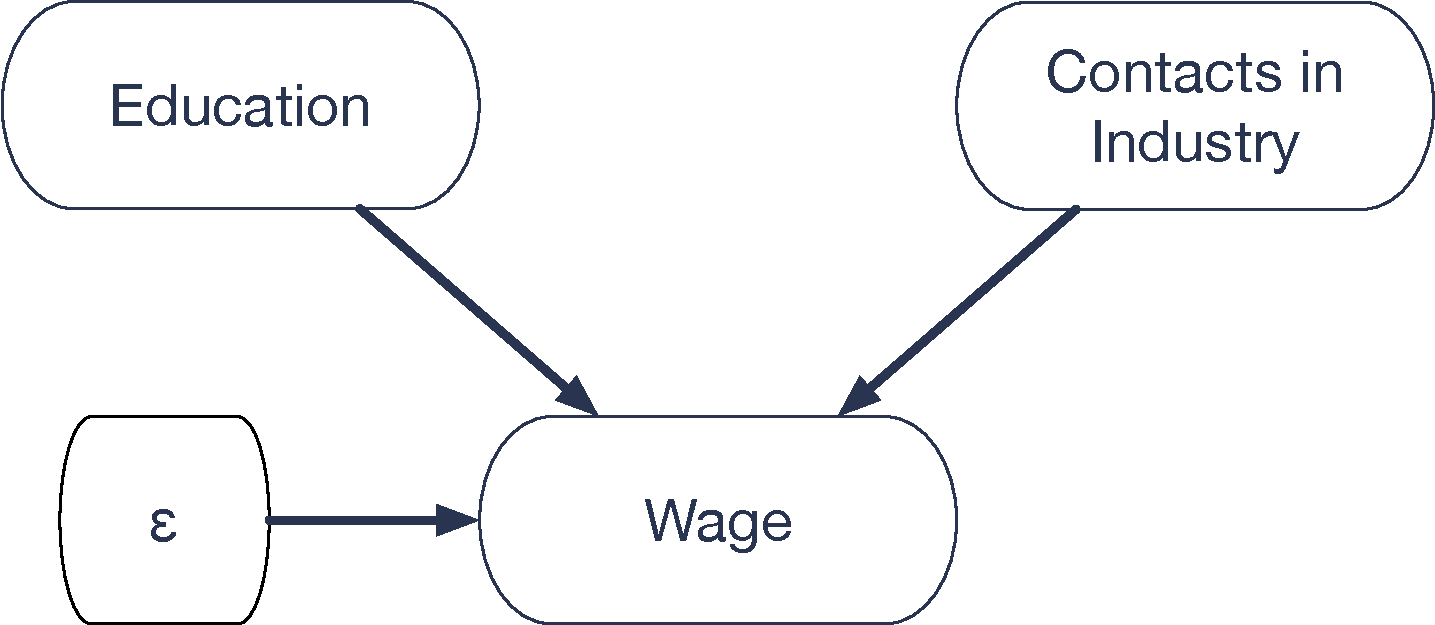
\includegraphics[width=0.49\linewidth]{images/assumed_right_hand_side}
    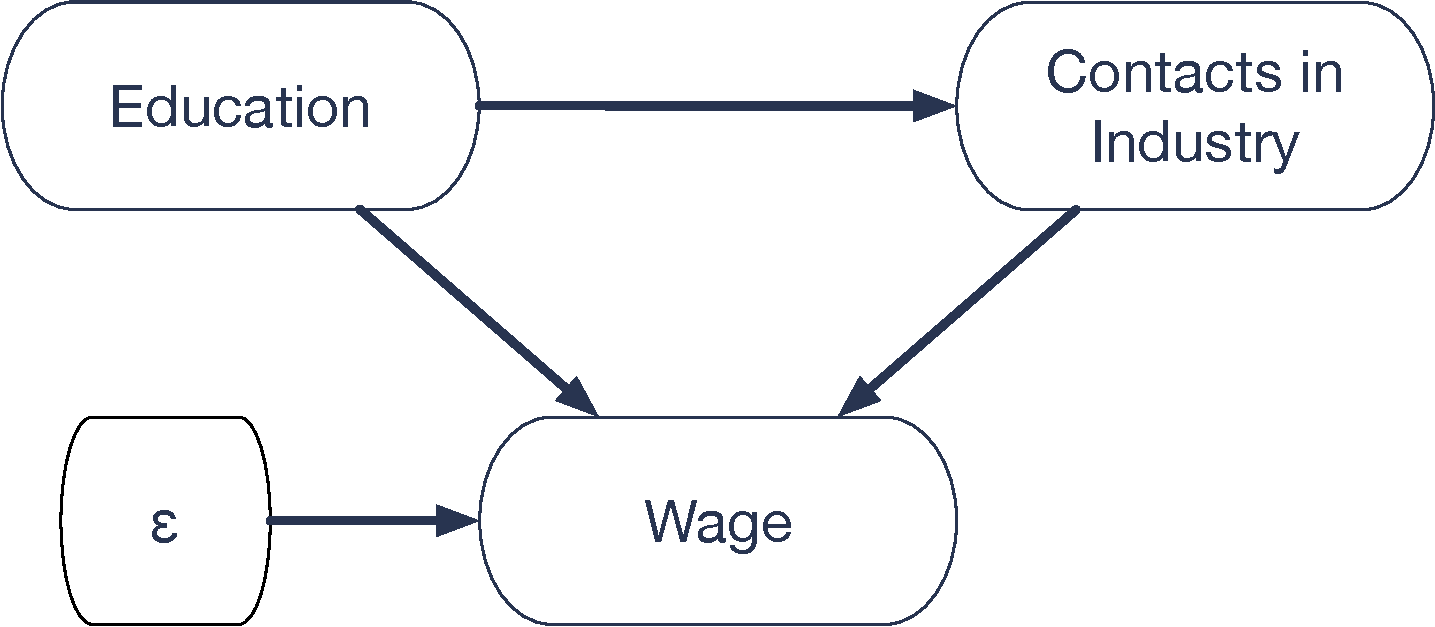
\includegraphics[width=0.49\linewidth]{images/true_right_hand_side}

    
    \note[item]{This last violation, is not actually a violation.  But
      it is a tricky situation that you need to be careful with.} 
    
    \note[item]{Let's say you record E and W as before, and you also
      have a third variable, $C$ the number of contacts a worker has in
      the same industry.}  
    
    \note[item]{Here's the issue.  We assume that the causal graph looks
      like the left one, but what if education causes you to have more
      contacts.  One of the main reasons for going to grad school is to
      build up your network.}  
    
    \note[item]{Can we use OLS to estimate the structural parameters?}
    
  \end{frame}


\begin{frame}
  \frametitle{Estimating the Structural Parameters}
  \note[item]{The answer is yes.  The same proof as before.  I can
    draw in W's background variable $\epsilon$.  There's no paths from
    here to $E$, so $E$ and $\epsilon$ are independent} 

  \begin{center}
    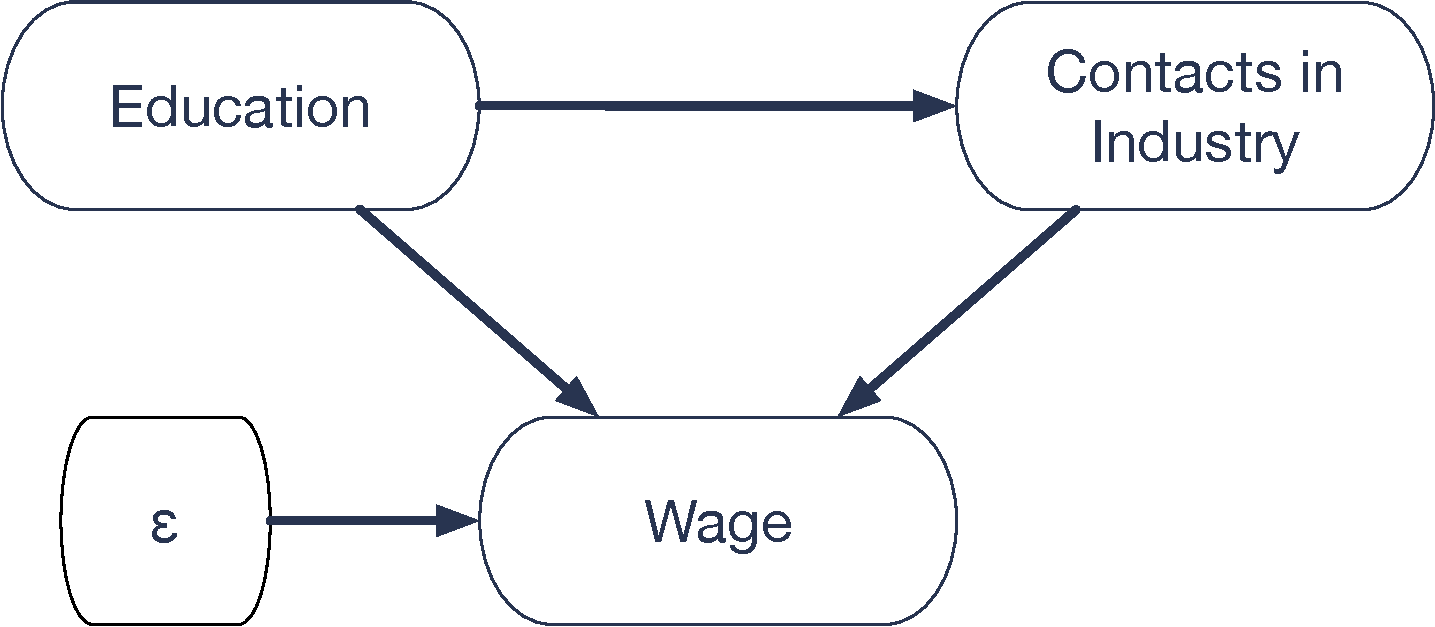
\includegraphics[height = 3cm]{images/true_right_hand_side}
  \end{center}
  
  Structural Equation: $W = \beta_0 + \beta_1 E + \beta_2 C + \epsilon \qquad (S)$ \\ 
  $\epsilon$ and $E$ have no common ancestors. \\ 
  $\implies \epsilon$ and $E$ are independent. \\ 
  $\implies cov(E,\epsilon) = 0$ \\ 
  $\implies$ OLS is consistent for $\beta_1$ \\ 
  
  \note[item]{OLS is consistent for $\beta_1$, but is this the
    coefficient you're interested in?}
\end{frame}


\begin{frame}
  \frametitle{Interpreting the Structural Coefficient}
  \note[item]{Let's think about what the interpretation is}
  
  $\beta_1$ - The expected increase in Wage, from getting an extra
  year of eduction, holding the number of industry contacts constant. 
  
  \note[item]{But that's strange formulation, right?  Go to school for
    a year, but don't make any contacts?  Of course, that would
    probably limit wages, but why would you do that?  The research
    question we're interested in isn't about specific parts of
    education, it's about a year of education as a whole.  So this is
    probably a bad idea.} 
  
\end{frame}



\begin{frame}[standout]
  \frametitle{Take Away}
  \centering
  Do not put outcome variables on the right hand side.
\end{frame}


\section{ Explanatory Modeling Wrap-Up}

\begin{frame}
  \frametitle{Take Aways}
  
  \note[item]{First, let me remind you that to do any explanatory
    modeling, you have to work inside a causal theory.  You could rush
    in, linear regressions blazing, but if you don't start with a
    causal theory, it's hard to know what your results mean.  At the
    least, it's worth your while to draw your causal graph, see if you
    can decide what your assumptions are.  It might tell you that you
    can use ols, it might require an advanced method like instrumental
    variables, or it might tell you that estimation is impossible, but
    at least you'll know.} 
  \begin{itemize}
  \item Explanatory modeling takes place inside a causal theory.
  \item The one-equation structural model is usually wrong.
  \item In special circumstances, advanced techniques can overcome
    omitted variables and reverse causality. 
    \begin{itemize}
    \item To learn more, try the instrumental variables and
      simultaneous equations chapters in \textit{Introductory
        Econometrics} (Wooldridge). 
    \end{itemize}
  \end{itemize}
\end{frame}

\end{document}
